% ICCV 2025 Paper Template

\documentclass[10pt,twocolumn,letterpaper]{article}

%%%%%%%%% PAPER TYPE  - PLEASE UPDATE FOR FINAL VERSION
%\usepackage{iccv}              % To produce the CAMERA-READY version
%\usepackage[review]{iccv}      % To produce the REVIEW version
\usepackage[pagenumbers]{iccv} % To force page numbers, e.g. for an arXiv version
\usepackage{subcaption}
\usepackage{booktabs} % for professional tables
\usepackage{amssymb}% http://ctan.org/pkg/amssymb
\usepackage{pifont}% http://ctan.org/pkg/pifont
\newcommand{\cmark}{\ding{51}}%
\newcommand{\xmark}{\ding{55}}%
% hyperref makes hyperlinks in the resulting PDF.
% If your build breaks (sometimes temporarily if a hyperlink spans a page)
% please comment out the following usepackage line and replace
% \usepackage{icml2025} with \usepackage[nohyperref]{icml2025} above.
\usepackage{makecell}
\usepackage{stackengine}
\usepackage{tikz}
\usepackage{pgfplots}
\pgfplotsset{compat=default}
\usetikzlibrary{pgfplots.groupplots}

% Import additional packages in the preamble file, before hyperref
%
% --- inline annotations
%
\newcommand{\red}[1]{{\color{red}#1}}
\newcommand{\todo}[1]{{\color{red}#1}}
\newcommand{\TODO}[1]{\textbf{\color{red}[TODO: #1]}}
% --- disable by uncommenting  
% \renewcommand{\TODO}[1]{}
% \renewcommand{\todo}[1]{#1}



\newcommand{\VLM}{LVLM\xspace} 
\newcommand{\ours}{PeKit\xspace}
\newcommand{\yollava}{Yo’LLaVA\xspace}

\newcommand{\thisismy}{This-Is-My-Img\xspace}
\newcommand{\myparagraph}[1]{\noindent\textbf{#1}}
\newcommand{\vdoro}[1]{{\color[rgb]{0.4, 0.18, 0.78} {[V] #1}}}
% --- disable by uncommenting  
% \renewcommand{\TODO}[1]{}
% \renewcommand{\todo}[1]{#1}
\usepackage{slashbox}
% Vectors
\newcommand{\bB}{\mathcal{B}}
\newcommand{\bw}{\mathbf{w}}
\newcommand{\bs}{\mathbf{s}}
\newcommand{\bo}{\mathbf{o}}
\newcommand{\bn}{\mathbf{n}}
\newcommand{\bc}{\mathbf{c}}
\newcommand{\bp}{\mathbf{p}}
\newcommand{\bS}{\mathbf{S}}
\newcommand{\bk}{\mathbf{k}}
\newcommand{\bmu}{\boldsymbol{\mu}}
\newcommand{\bx}{\mathbf{x}}
\newcommand{\bg}{\mathbf{g}}
\newcommand{\be}{\mathbf{e}}
\newcommand{\bX}{\mathbf{X}}
\newcommand{\by}{\mathbf{y}}
\newcommand{\bv}{\mathbf{v}}
\newcommand{\bz}{\mathbf{z}}
\newcommand{\bq}{\mathbf{q}}
\newcommand{\bff}{\mathbf{f}}
\newcommand{\bu}{\mathbf{u}}
\newcommand{\bh}{\mathbf{h}}
\newcommand{\bb}{\mathbf{b}}

\newcommand{\rone}{\textcolor{green}{R1}}
\newcommand{\rtwo}{\textcolor{orange}{R2}}
\newcommand{\rthree}{\textcolor{red}{R3}}
\usepackage{amsmath}
%\usepackage{arydshln}
\DeclareMathOperator{\similarity}{sim}
\DeclareMathOperator{\AvgPool}{AvgPool}

\newcommand{\argmax}{\mathop{\mathrm{argmax}}}     



% It is strongly recommended to use hyperref, especially for the review version.
% hyperref with option pagebackref eases the reviewers' job.
% Please disable hyperref *only* if you encounter grave issues, 
% e.g. with the file validation for the camera-ready version.
%
% If you comment hyperref and then uncomment it, you should delete *.aux before re-running LaTeX.
% (Or just hit 'q' on the first LaTeX run, let it finish, and you should be clear).
\definecolor{iccvblue}{rgb}{0.21,0.49,0.74}
\usepackage[pagebackref,breaklinks,colorlinks,allcolors=iccvblue]{hyperref}

%%%%%%%%% PAPER ID  - PLEASE UPDATE
\def\paperID{*****} % *** Enter the Paper ID here
\def\confName{ICCV}
\def\confYear{2025}

%%%%%%%%% TITLE - PLEASE UPDATE
\title{PixFoundation: Are We Heading in the Right Direction with \\Pixel-level Vision Foundation Models?}

%%%%%%%%% AUTHORS - PLEASE UPDATE
\author{Mennatullah Siam\\
University of British Columbia\\
BC, Canada\\
{\tt\small mennatullah.siam@ubc.ca}
% For a paper whose authors are all at the same institution,
% omit the following lines up until the closing ``}''.
% Additional authors and addresses can be added with ``\and'',
% just like the second author.
% To save space, use either the email address or home page, not both
}

\begin{document}
\maketitle

\begin{abstract}
\begin{abstract}  
Test time scaling is currently one of the most active research areas that shows promise after training time scaling has reached its limits.
Deep-thinking (DT) models are a class of recurrent models that can perform easy-to-hard generalization by assigning more compute to harder test samples.
However, due to their inability to determine the complexity of a test sample, DT models have to use a large amount of computation for both easy and hard test samples.
Excessive test time computation is wasteful and can cause the ``overthinking'' problem where more test time computation leads to worse results.
In this paper, we introduce a test time training method for determining the optimal amount of computation needed for each sample during test time.
We also propose Conv-LiGRU, a novel recurrent architecture for efficient and robust visual reasoning. 
Extensive experiments demonstrate that Conv-LiGRU is more stable than DT, effectively mitigates the ``overthinking'' phenomenon, and achieves superior accuracy.
\end{abstract}  
\end{abstract}

\section{Introduction}
\section{Introduction}


\begin{figure}[t]
\centering
\includegraphics[width=0.6\columnwidth]{figures/evaluation_desiderata_V5.pdf}
\vspace{-0.5cm}
\caption{\systemName is a platform for conducting realistic evaluations of code LLMs, collecting human preferences of coding models with real users, real tasks, and in realistic environments, aimed at addressing the limitations of existing evaluations.
}
\label{fig:motivation}
\end{figure}

\begin{figure*}[t]
\centering
\includegraphics[width=\textwidth]{figures/system_design_v2.png}
\caption{We introduce \systemName, a VSCode extension to collect human preferences of code directly in a developer's IDE. \systemName enables developers to use code completions from various models. The system comprises a) the interface in the user's IDE which presents paired completions to users (left), b) a sampling strategy that picks model pairs to reduce latency (right, top), and c) a prompting scheme that allows diverse LLMs to perform code completions with high fidelity.
Users can select between the top completion (green box) using \texttt{tab} or the bottom completion (blue box) using \texttt{shift+tab}.}
\label{fig:overview}
\end{figure*}

As model capabilities improve, large language models (LLMs) are increasingly integrated into user environments and workflows.
For example, software developers code with AI in integrated developer environments (IDEs)~\citep{peng2023impact}, doctors rely on notes generated through ambient listening~\citep{oberst2024science}, and lawyers consider case evidence identified by electronic discovery systems~\citep{yang2024beyond}.
Increasing deployment of models in productivity tools demands evaluation that more closely reflects real-world circumstances~\citep{hutchinson2022evaluation, saxon2024benchmarks, kapoor2024ai}.
While newer benchmarks and live platforms incorporate human feedback to capture real-world usage, they almost exclusively focus on evaluating LLMs in chat conversations~\citep{zheng2023judging,dubois2023alpacafarm,chiang2024chatbot, kirk2024the}.
Model evaluation must move beyond chat-based interactions and into specialized user environments.



 

In this work, we focus on evaluating LLM-based coding assistants. 
Despite the popularity of these tools---millions of developers use Github Copilot~\citep{Copilot}---existing
evaluations of the coding capabilities of new models exhibit multiple limitations (Figure~\ref{fig:motivation}, bottom).
Traditional ML benchmarks evaluate LLM capabilities by measuring how well a model can complete static, interview-style coding tasks~\citep{chen2021evaluating,austin2021program,jain2024livecodebench, white2024livebench} and lack \emph{real users}. 
User studies recruit real users to evaluate the effectiveness of LLMs as coding assistants, but are often limited to simple programming tasks as opposed to \emph{real tasks}~\citep{vaithilingam2022expectation,ross2023programmer, mozannar2024realhumaneval}.
Recent efforts to collect human feedback such as Chatbot Arena~\citep{chiang2024chatbot} are still removed from a \emph{realistic environment}, resulting in users and data that deviate from typical software development processes.
We introduce \systemName to address these limitations (Figure~\ref{fig:motivation}, top), and we describe our three main contributions below.


\textbf{We deploy \systemName in-the-wild to collect human preferences on code.} 
\systemName is a Visual Studio Code extension, collecting preferences directly in a developer's IDE within their actual workflow (Figure~\ref{fig:overview}).
\systemName provides developers with code completions, akin to the type of support provided by Github Copilot~\citep{Copilot}. 
Over the past 3 months, \systemName has served over~\completions suggestions from 10 state-of-the-art LLMs, 
gathering \sampleCount~votes from \userCount~users.
To collect user preferences,
\systemName presents a novel interface that shows users paired code completions from two different LLMs, which are determined based on a sampling strategy that aims to 
mitigate latency while preserving coverage across model comparisons.
Additionally, we devise a prompting scheme that allows a diverse set of models to perform code completions with high fidelity.
See Section~\ref{sec:system} and Section~\ref{sec:deployment} for details about system design and deployment respectively.



\textbf{We construct a leaderboard of user preferences and find notable differences from existing static benchmarks and human preference leaderboards.}
In general, we observe that smaller models seem to overperform in static benchmarks compared to our leaderboard, while performance among larger models is mixed (Section~\ref{sec:leaderboard_calculation}).
We attribute these differences to the fact that \systemName is exposed to users and tasks that differ drastically from code evaluations in the past. 
Our data spans 103 programming languages and 24 natural languages as well as a variety of real-world applications and code structures, while static benchmarks tend to focus on a specific programming and natural language and task (e.g. coding competition problems).
Additionally, while all of \systemName interactions contain code contexts and the majority involve infilling tasks, a much smaller fraction of Chatbot Arena's coding tasks contain code context, with infilling tasks appearing even more rarely. 
We analyze our data in depth in Section~\ref{subsec:comparison}.



\textbf{We derive new insights into user preferences of code by analyzing \systemName's diverse and distinct data distribution.}
We compare user preferences across different stratifications of input data (e.g., common versus rare languages) and observe which affect observed preferences most (Section~\ref{sec:analysis}).
For example, while user preferences stay relatively consistent across various programming languages, they differ drastically between different task categories (e.g. frontend/backend versus algorithm design).
We also observe variations in user preference due to different features related to code structure 
(e.g., context length and completion patterns).
We open-source \systemName and release a curated subset of code contexts.
Altogether, our results highlight the necessity of model evaluation in realistic and domain-specific settings.






\section{Related work}
\putsec{related}{Related Work}

\noindent \textbf{Efficient Radiance Field Rendering.}
%
The introduction of Neural Radiance Fields (NeRF)~\cite{mil:sri20} has
generated significant interest in efficient 3D scene representation and
rendering for radiance fields.
%
Over the past years, there has been a large amount of research aimed at
accelerating NeRFs through algorithmic or software
optimizations~\cite{mul:eva22,fri:yu22,che:fun23,sun:sun22}, and the
development of hardware
accelerators~\cite{lee:cho23,li:li23,son:wen23,mub:kan23,fen:liu24}.
%
The state-of-the-art method, 3D Gaussian splatting~\cite{ker:kop23}, has
further fueled interest in accelerating radiance field
rendering~\cite{rad:ste24,lee:lee24,nie:stu24,lee:rho24,ham:mel24} as it
employs rasterization primitives that can be rendered much faster than NeRFs.
%
However, previous research focused on software graphics rendering on
programmable cores or building dedicated hardware accelerators. In contrast,
\name{} investigates the potential of efficient radiance field rendering while
utilizing fixed-function units in graphics hardware.
%
To our knowledge, this is the first work that assesses the performance
implications of rendering Gaussian-based radiance fields on the hardware
graphics pipeline with software and hardware optimizations.

%%%%%%%%%%%%%%%%%%%%%%%%%%%%%%%%%%%%%%%%%%%%%%%%%%%%%%%%%%%%%%%%%%%%%%%%%%
\myparagraph{Enhancing Graphics Rendering Hardware.}
%
The performance advantage of executing graphics rendering on either
programmable shader cores or fixed-function units varies depending on the
rendering methods and hardware designs.
%
Previous studies have explored the performance implication of graphics hardware
design by developing simulation infrastructures for graphics
workloads~\cite{bar:gon06,gub:aam19,tin:sax23,arn:par13}.
%
Additionally, several studies have aimed to improve the performance of
special-purpose hardware such as ray tracing units in graphics
hardware~\cite{cho:now23,liu:cha21} and proposed hardware accelerators for
graphics applications~\cite{lu:hua17,ram:gri09}.
%
In contrast to these works, which primarily evaluate traditional graphics
workloads, our work focuses on improving the performance of volume rendering
workloads, such as Gaussian splatting, which require blending a huge number of
fragments per pixel.

%%%%%%%%%%%%%%%%%%%%%%%%%%%%%%%%%%%%%%%%%%%%%%%%%%%%%%%%%%%%%%%%%%%%%%%%%%
%
In the context of multi-sample anti-aliasing, prior work proposed reducing the
amount of redundant shading by merging fragments from adjacent triangles in a
mesh at the quad granularity~\cite{fat:bou10}.
%
While both our work and quad-fragment merging (QFM)~\cite{fat:bou10} aim to
reduce operations by merging quads, our proposed technique differs from QFM in
many aspects.
%
Our method aims to blend \emph{overlapping primitives} along the depth
direction and applies to quads from any primitive. In contrast, QFM merges quad
fragments from small (e.g., pixel-sized) triangles that \emph{share} an edge
(i.e., \emph{connected}, \emph{non-overlapping} triangles).
%
As such, QFM is not applicable to the scenes consisting of a number of
unconnected transparent triangles, such as those in 3D Gaussian splatting.
%
In addition, our method computes the \emph{exact} color for each pixel by
offloading blending operations from ROPs to shader units, whereas QFM
\emph{approximates} pixel colors by using the color from one triangle when
multiple triangles are merged into a single quad.



\section{Method and benchmarks}
\label{sec:method}
\begin{figure*}[t]
\centering
\includegraphics[width=\textwidth]{images/pixelmllms_failures/failures_pixmllms_3.drawio.pdf}
\vspace{-2em}
\caption{Second shortcoming of pixel-level MLLMs is the degraded performance in pixel-level visual grounding in certain models. The predicted segmentation is highlighted in red.} 
\label{fig:shortcoming3}
\vspace{-1em}
\end{figure*}

\begin{figure}[t]
\centering
\includegraphics[width=0.5\textwidth]{images/pixelmllms_failures/failures_pixmllms_2.drawio.pdf}
\vspace{-2em}
\caption{Third shortcoming of pixel-level MLLMs is the degraded performance in instruction following, where the question is instructing the model to generate one letter from the options.} 
\label{fig:shortcoming2}
\vspace{-1em}
\end{figure}

In this section, we describe our two benchmarks and probing techniques for pixel-level MLLMs and MLLMs that were not trained with pixel-level grounding supervision.
\subsection{Benchmarks}
\textbf{PixMMVP benchmark:} We build upon the recently released MMVP~\cite{tong2024eyes} which identified clip blind pairs and used them to build a challenging benchmark with the corresponding questions and choices for 300 images. We augment the aforementioned dataset and manually annotate each question with the corresponding object of interest referring expression, e.g. an elderly person or the butterfly's feet. There are seven questions only that are not designed to inquire about a specific object in the scene, which are excluded. Examples include questions inquiring on the view direction of the camera which are not tied to a specific entity. Our manual referring expression annotations are as fine-grained as possible. These expressions correspond to what needs to be grounded in the image to answer the question. Afterwards, we manually label these objects of interest with polygonal annotations using the VGG annotator~\cite{dutta2016via}.

\textbf{PixCV-Bench benchmark:} For this benchmark we build upon the 2D component of the recently released CV-Bench~\cite{tong2024cambrian}. We specifically select the 2D component, since they are sourced from segmentation datasets (i.e., ADE20K~\cite{zhou2017scene} and COCO~\cite{lin2014microsoft}), which can be used in our proposed benchmark. However, the publicly released CV-Bench does not identify the objects in question and their corresponding segmentation. As such we use GPT-4o to parse the questions and identify the objects of interest automatically, followed by manual inspection and correction. Specifically, we collect the classes in each image from the corresponding dataset and construct a list of class choices ``1. $<$CLS1$>$, 2. $<$CLS2$>$, ...''. Then we prompt GPT-4o with the following, \textit{``Provide number only as an answer. Identify the objects of interest in the following question: $<$QUESTION$>$ ? 1. $<$CLS1$>$, 2. $<$CLS2$>$, ... ''.}  This provides us with the categories per question that highlights the objects of interest. While seemingly these are categorical annotations not referring expressions, certain scenarios in CV-Bench are different. Specifically, in the relative positioning task all the questions that include an object highlighted by a red box in the image are annotated with the referring expression, ``(annotated by the red box)'', beyond simple categorical annotations.

Afterwards, we use the selected categories from GPT-4o to retrieve the corresponding segmentation mask/s per image. Furthermore, we use a custom annotation tool to manually filter the objects in the question, e.g. selecting only the object mask annotated by the red box when referred to it and filtering out the other instances for that same class. Another example that needs manual filtration when the class in question is a broader category than what is inquired upon, e.g., ``Pendant Lamp'' which is under the category of ``Lamp'' in ADE20K. In such a case, we filter out the masks of other types such as ``Table Lamp''. Moreover, we identify missing annotations in rare occasions that require additional intervention and manually annotate these missing objects. We provide the final PixCV-Bench with referring expressions and their segmentation annotations that can be used to evaluate the grounding ability in relation to the original VQA task. Appendix~\ref{app:impdetails} provides visual examples from our benchmarks.

\subsection{A Pixel-level MLLMs study}

We utilize the two proposed benchmarks, PixMMVP and PixCV-Bench, to evaluate how the current trend in pixel-level MLLMs that relies on training with grounding supervision perform in such challenging tasks. Furthermore, we inspect the failures of these pixel-level MLLMs and explore simple approaches to pixel-level understanding from MLLMs that overcome the previous shortcomings. %We aim to answer two major research questions in our study; ``How do Pixel-level MLLMs perform in challenging pixel-level visual grounding tasks?'' and ``Whether grounding can be extracted from MLLMs that were not necessarily trained with full supervision as a simpler but more powerful means? and When does that grounding emerge?''

\textbf{Pixel-level MLLMs shortcomings.} We highlight the failures for the current state-of-the-art pixel-level MLLMs through three probing techniques. First, we highlight the degraded performance in VQA from most of the pixel-level MLLMs that are trained with pixel-level grounding supervision. We use for that the following prompt, \textit{``$<$IMG$>$$<$QUESTION$>$? $<$OPTION1$>$ $<$OPTION2$>$...''}, as shown in Figure~\ref{fig:shortcoming1}. Certain pixel-level MLLMs tend to answer the aforementioned question while outputting a corresponding segmentation mask/s for the objects of interest. Notably, the worst two models in this task, LISA~\cite{lai2024lisa} and GLAMM~\cite{rasheed2024glamm}, are not able to provide an answer and rather refer to a segmentation mask. On the other hand, OMG-Llava~\cite{zhang2024omg} shows better ability in VQA.%, yet the answer is not necessarily the correct one.

The second shortcoming we discuss is their degraded ability to visually ground objects. Surprisingly, although they were trained with pixel-level grounding supervision, not all of these models show superior grounding performance. Figure~\ref{fig:shortcoming3} shows the second prompt to generate a segmentation mask for the ground-truth referring expression. The purpose of this probing is to understand whether the failure in these models is purely on the VQA task, or its inability to ground the objects of interest in the corresponding question or both. Figure~\ref{fig:shortcoming3} shows the worst two models in this aspect, which are GLAMM, the region captioning variant, and Llava-G. Both fail to segment the specific object in question, while OMG-Llava shows better performance.

Third, we highlight another shortcoming, where these MLLMs exhibit degraded ability to follow instructions. In order to probe this, we use the following prompt: \textit{``$<$IMG$>$$<$QUESTION$>$? a.$<$OPTION1$>$ b.$<$OPTION2$>$... Answer with the option's letter from the given.''} Figure~\ref{fig:shortcoming2} shows an example with the answers from the worst two models in this aspect which are LISA~\cite{lai2024lisa} and Llava-G~\cite{zhang2025llava}. Both are incapable of following the instruction, yet Llava-G tries to tackle the question unlike LISA. On the other hand, OMG-Llava shows better ability to follow the instruction and answer the question. 

\textbf{Baselines and upper bounds.} In addition to evaluating state-of-the-art pixel-level MLLMs, we propose two baselines and one upper bound. The first of which is inspired by a concurrent work~\cite{cao2024emerging} that identified the emergent grounding in multi-modal large language models without the need for any pixel-level grounding supervision. Specifically, we use their attend and segment meta architecture as one of our baselines. However, we are the first to discuss when does such grounding emerge in these models. We identify an interesting connection between the identified output tokens and the output grounding from the attention maps that gives insights on how these models reason. 

The attend and segment meta-architecture extracts the raw attention map for the $i^{th}$ output token, $A_i \in [0, 1]^{n_{\text{layer}} \times n_{\text{head}} \times (x+hw+y+i-1)}$, where $n_{\text{layer}}, n_{\text{head}}$  are the number of layers and heads, resp. Then, $x,y$ are the number of input language tokens before and after the visual tokens respectively, while $hw$ are the height and width of the input image. Only the attention corresponding to the visual tokens of length $hw$ are used, and these attention maps are averaged across the layers and heads, resulting in $\bar{A}_i \in [0, 1]^{h \times w}$. This is further normalized across all the output, $\tilde{A}_i = \bar{A}_i - \frac{1}{N} \sum_{j=1}^{N}{\bar{A}_j}$ for $N$ output tokens. The attend and segment depends on using spaCy natural language processing tool~\cite{spaCy} to identify the noun phrases and associate them to the ground-truth referring expressions. Thus, the spaCy embeddings closest to the ground-truth expression are used in the mask selection. This is followed by extracting the maximum attention point to feed into SAM~\cite{kirillov2023segment} as a point prompt.

%\begin{table*}[t]
%\centering
%\begin{tabular}{lc|cccc|c}
%\hline
%\textbf{Method} & \textbf{PixGr. Train} & \multicolumn{4}{|c|}{\textbf{MMVP \& PixMMVP}}  \\ 
%                &                  & $\mathcal{A}\dagger$  & $\mathcal{A}$ & $\mathcal{M}\dagger$ & $\mathcal{M}$ & $\mathcal{S}$\\\hline
%Llava 1.5 (7B)~\cite{liu2024visual}  &   \xmark      &     \textbf{28.7}       & \textbf{28.0}      &     -      &     -     & -\\
%Llava 1.5 (13B)~\cite{liu2024visual} &   \xmark      &     \textbf{39.3}       & \textbf{30.0}      &     -      &     -     & -\\
%Cambrian (8B)*~\cite{tong2024cambrian}  &   \xmark   & \textbf{52.0}  & \textbf{52.0} &     -      &     -     & -\\
%OMG Llava (7B)**~\cite{zhang2024omg}  &   \checkmark   &     12.0       & 12.0      &    17.8    &     38.0  & 18.2\\
%GLAMM (7B)~\cite{rasheed2024glamm} &   \checkmark    &      1.3         &   2.7     &    \textbf{31.5}    &     \textbf{47.4}  & 5.1\\
%GLAMM - RegCap (7B)~\cite{rasheed2024glamm} &   \checkmark    &      12.7              &    6.7    &    14.5    &     18.6  & 15.1\\
%LISA (7B)~\cite{lai2024lisa}       &   \checkmark    &       7.3              &    -      &     18.1      &    42.9   & 12.5\\
%Llava-G (7B)~\cite{zhang2025llava}    &    \checkmark   &       9.3             &    -      &     17.8   &     13.5  & 12.2\\
%
%Llava 1.5 (7B) + (a+s)~\cite{cao2024emerging}  &  \xmark &      \textbf{28.7}       & \textbf{28.0} &   11.1  &  11.2 & 16.1 \\ 
%Llava 1.5 (13B) + (a+s)~\cite{cao2024emerging} &  \xmark &        \textbf{39.3}  &    \textbf{30.0}   &    9.8  &  11.4 & 17.7\\ 
%Cambrian (8B)* + (a+s)~\cite{cao2024emerging}  &  \xmark &      \textbf{52.0}            & \textbf{52.0}  &   14.3  &  15.1 & 23.4 \\ \hline
%
%PixFoundation (Llava (7B)) (Ours)    & \xmark  &     \textbf{28.7}       & \textbf{28.0} &  16.9  & 18.8 & \textbf{22.7}\\ 
%PixFoundation (Llava (13B)) (Ours)    & \xmark  &    \textbf{39.3}  &     \textbf{30.0}  &   \textbf{14.4} & \textbf{18.2} & \textbf{24.9}\\ 
%PixFoundation (Cambrian (8B)*) (Ours)    & \xmark  &  \textbf{52.0} &  \textbf{52.0}  &  \textbf{17.2}  & \textbf{18.9} & \textbf{27.7} \\ \hline
%\multicolumn{7}{l}{\textbf{Upper Bound - Oracle Selection}} \\ \hline
%PixFoundation$\dagger$ (Llava (7B)) (Ours)    & \xmark  &     28.7       & 28.0 &  \textbf{\textcolor{red}{26.1}}   & \textbf{\textcolor{red}{38.0}}   & \textcolor{red}{\textbf{32.7}}\\ 
%PixFoundation$\dagger$ (Llava (13B)) (Ours)    & \xmark  &    39.3  &   30.0  &    \textbf{\textcolor{red}{23.6}} &   \textbf{\textcolor{red}{38.2}} & \textcolor{red}{\textbf{38.7}}\\ 
%PixFoundation$\dagger$ (Cambrian (8B)*) (Ours)    & \xmark  & 52.0  & 52.0 & \textbf{\textcolor{red}{52.0}}  & \textbf{\textcolor{red}{56.1}} &  \textcolor{red}{\textbf{54.0}}\\ \hline
%\end{tabular}
%\caption{\textbf{PixMMVP} benchmark evaluation of pixel-level MLLMs and baselines. We evaluate the VQA accuracy in the first and third probing (i.e., $\mathcal{A}\dagger$ and $\mathcal{A}$ resp.). Additionally, we evaluate pixel-level visual grounding with output segmentation in the first two probing (i.e., $\mathcal{M}\dagger$ and $\mathcal{M}$ resp.). *, **: models using Llama 3 (8B) and InterLM2 (7B) respectively, unlike the rest that are relying on Vicuna (7B and 13B) for the base LLM. - : indicates either the model can not be evaluated in that setting, or has low results below 1\% showing complete failure in that setting. $\mathcal{S}$: denotes the score of the MLLM that is the harmonic mean of $\text{max}(\mathcal{A}, \mathcal{A}\dagger)$ and $\text{max}(\mathcal{M}, \mathcal{M}\dagger)$. PixGr. Train: pixel-level grounding training. The oracle results are highlighted in red, and the best in each variant (7B, 13B, and 8B) are bolded. }
%\label{tab:pixmmvp}
%\end{table*}

%\begin{table*}[t]
%\centering
%\begin{tabular}{lc|cccc|c}
%\hline
%\textbf{Method} & \textbf{PixGr. Train} & \multicolumn{4}{|c|}{\textbf{PixMMVP}}  \\ 
%                &                  & $\mathcal{A}\dagger$  & $\mathcal{A}$ & $\mathcal{M}\dagger$ & $\mathcal{M}$ & $\mathcal{S}$\\\hline
%Llava 1.5 (7B)~\cite{liu2024visual}  &   \xmark      &     \textbf{27.3}       & \textbf{28.0}      &     -      &     -     & -\\
%Llava 1.5 (13B)~\cite{liu2024visual} &   \xmark      &   \textbf{39.3}        &  \textbf{30}     &     -      &     -     & -\\
%Cambrian (8B)*~\cite{tong2024cambrian}  &   \xmark   & \textbf{52.0}  & \textbf{52.0} &     -      &     -     & -\\
%OMG Llava (7B)**~\cite{zhang2024omg}  &   \checkmark   &     12.0       & 12.0      &    17.8    &     38.0  & 18.2\\
%GLAMM (7B)~\cite{rasheed2024glamm} &   \checkmark    &      1.3         &   2.7     &    \textbf{31.5}    &     \textbf{47.4}  & 5.1\\
%GLAMM - RegCap (7B)~\cite{rasheed2024glamm} &   \checkmark    &      12.7              &    6.7    &    14.5    &     18.6  & 15.1\\
%LISA (7B)~\cite{lai2024lisa}       &   \checkmark    &       7.3              &    -      &     18.1      &    42.9   & 12.5\\
%Llava-G (7B)~\cite{zhang2025llava}    &    \checkmark   &       9.3             &    -      &     17.8   &     13.5  & 12.2\\
%
%Llava 1.5 (7B) + (a+s)~\cite{cao2024emerging}  &  \xmark &  \textbf{27.3}       & \textbf{28.0}      &   11.1  &  11.2 &  16.0\\ 
%Llava 1.5 (13B) + (a+s)~\cite{cao2024emerging} &  \xmark &  \textbf{39.3}        &  \textbf{30}    &  9.8   & 11.4  & 17.7\\ 
%Cambrian (8B)* + (a+s)~\cite{cao2024emerging}  &  \xmark &      \textbf{52.0}            & \textbf{52.0}  &   14.3  &  15.1 & 23.4 \\ \hline
%
%% Old approach using Cambrian
%%PixFoundation (Llava (7B)) (Ours)    & \xmark  &    \textbf{27.3}       & \textbf{28.0}      &  16.9  & 18.8 & \textbf{22.5}\\ 
%%PixFoundation (Llava (13B)) (Ours)    & \xmark  &   \textbf{39.3}        &  \textbf{30}     &  \textbf{14.4}  & \textbf{18.2} & \textbf{24.9} \\ 
%%PixFoundation (Cambrian (8B)*) (Ours)    & \xmark  &  \textbf{52.0} &  \textbf{52.0}  &  \textbf{17.2}  & \textbf{18.9} & \textbf{27.7} \\ \hline
%
%% new approach using GPT
%PixFoundation (Llava (7B)) (Ours)    & \xmark  &    \textbf{27.3}       & \textbf{28.0}      & 18.8  & 25.9 & \textbf{26.9}\\ 
%PixFoundation (Llava (13B)) (Ours)    & \xmark  &   \textbf{39.3}        &  \textbf{30}     &  \textbf{16.9}  & \textbf{25.0} &  \textbf{30.6}\\ 
%PixFoundation (Cambrian (8B)*) (Ours)    & \xmark  &  \textbf{52.0} &  \textbf{52.0}  &  \textbf{29.6}  &  \textbf{30.3} & \textbf{38.3} \\ \hline
%
%\multicolumn{7}{l}{\textbf{Upper Bound - Oracle Selection}} \\ \hline
%PixFoundation$\dagger$ (Llava (7B)) (Ours)    & \xmark  &    27.3  & 28.0  &  \textbf{\textcolor{red}{26.1}}   & \textbf{\textcolor{red}{38.0}}   & \textcolor{red}{\textbf{32.2}}\\ 
%PixFoundation$\dagger$ (Llava (13B)) (Ours)    & \xmark  &    39.3        &  30 &  \textbf{\textcolor{red}{23.6}}  &  \textbf{\textcolor{red}{38.2}} & \textbf{\textcolor{red}{38.7}}\\ 
%PixFoundation$\dagger$ (Cambrian (8B)*) (Ours)    & \xmark  & 52.0  & 52.0 & \textbf{\textcolor{red}{52.0}}  & \textbf{\textcolor{red}{56.1}} &  \textcolor{red}{\textbf{54.0}}\\ \hline
%\end{tabular}
%\caption{\textbf{PixMMVP} benchmark evaluation of pixel-level MLLMs and baselines. We evaluate the VQA accuracy in the first and third probing (i.e., $\mathcal{A}\dagger$ and $\mathcal{A}$ resp.). Additionally, we evaluate pixel-level visual grounding with output segmentation in the first two probing (i.e., $\mathcal{M}\dagger$ and $\mathcal{M}$ resp.). *, **: models using Llama 3 (8B) and InterLM2 (7B) respectively, unlike the rest that are relying on Vicuna (7B and 13B) for the base LLM. - : indicates either the model can not be evaluated in that setting, or has low results below 1\% showing complete failure in that setting. $\mathcal{S}$: denotes the score of the MLLM that is the harmonic mean of $\text{max}(\mathcal{A}, \mathcal{A}\dagger)$ and $\text{max}(\mathcal{M}, \mathcal{M}\dagger)$. PixGr. Train: pixel-level grounding training. The oracle results are highlighted in red, and the best in each variant (7B, 13B, and 8B) are bolded. }
%\label{tab:pixmmvp}
%\end{table*}

For our baseline and upper bound, we build upon the previous pipeline and build an \textit{oracle} upper bound and an \textit{automatic} baseline. We introduce two main modifications to account for our observation that the correct grounding can occur with different output tokens describing the object not necessarily aligning with the exact ground-truth expression. The first modification is to go through all the potential output tokens without relying on spaCy embeddings. In the \textit{oracle} we rely on the ground-truth mask to select the correct token and its corresponding attention map with highest intersection over union as an upper bound. The \textit{automatic} baseline uses a simple but powerful mechanism where we overlay the predicted masks on the original image to highlight the potential object of interest. This is followed by feeding these images to a multi-modal LLM inquiring on which is best in highlighting this object. Specifically, we use the following prompt \textit{``Select the image that has $<$EXPR$>$ best highlighted in red color than the others? Answer with a number from 1 to $<$N$>$ and mention the number only. $<$IMG$>$''}, where  $<$EXPR$>$ and $<$IMG$>$ are the ground-truth expression and the image tokens respectively. In our automatic baseline we rely on GPT-4o for the mask selection. The second modification, since SAM has a good understanding of point prompting ambiguity, we process three potential output masks for each prompt instead of one only. This enables us to utilize the power of SAM in identifying fine-grained objects and referring expressions that tends to surpass what other MLLMs do, even those trained with pixel-level grounding supervision. %These baselines serve the main purpose that the correct grounding is already embedded in these MLLMs without any grounding supervision and the \textit{oracle} upper bound shows it surpasses any other MLLM with a significant margin. Thus, our proposed benchmarks and baselines confirm that pixel-level grounding is already embedded in such MLLMs and there is still plenty of opportunity to improve the grounding output further if equipped with the right tool to identify when grounding emerges.

%\begin{table*}[t]
%\centering
%\begin{tabular}{lc|cccc|c}
%\hline
%\textbf{Method}                     & \textbf{PixGr. Train} & \multicolumn{4}{|c|}{\textbf{CV-Bench \& PixCV-Bench}} \\
%                                    &                  & $\mathcal{A}\dagger$  & $\mathcal{A}$ & $\mathcal{M}$ & $\mathcal{M}\dagger$ & $\mathcal{S}$\\\hline
%%LLava 1.5 (7B)                      & \xmark           & \textbf{52.6/66.2/59.4} & \textbf{55.0/67.5/61.3} &     -     &     -      & -\\
%%LLava 1.5 (13B)                     &  \xmark          & \textbf{51.8/65.6/59.1} & \textbf{55.6/68.7/62.1} &     -     &    -       & -\\
%Llava 1.5 (7B)~\cite{liu2024visual}  & \xmark           & 16.7/14.7/15.7 & \textbf{54.2/66.5/60.4} &     -     &     -      & -\\
%Llava 1.5 (13B)~\cite{liu2024visual}  &  \xmark          & \textbf{14.6/16.7/15.6} & \textbf{55.6/67.1/61.3} &     -     &    -       & -\\
%Cambrian (8B)*~\cite{tong2024cambrian}&\xmark          & \textbf{55.7/68.7/62.2} &  \textbf{65.2/79.1/72.2}  &     -     &     -   & -\\
%OMG Llava (7B)**~\cite{zhang2024omg}    &   \checkmark    & 9.2/14.7/12.0 & 36.8/47.4/42.1 &   -       &   50.5  & \textbf{45.9}\\%OMG LLava changed
%GLAMM (7B)~\cite{rasheed2024glamm}    &    \checkmark   &      -         &      -         &   \textbf{30.2}    & \textbf{51.9}   & -\\
%GLAMM - RCap (7B)~\cite{rasheed2024glamm} &   \checkmark    & \textbf{22.8/32.8/27.8} & 46.8/62.0/54.4 &  3.6      &  7.4  & 13.0\\
%LISA (7B)~\cite{lai2024lisa}       &   \checkmark    & 1.9/5.5/3.7  &       -        &   16.8    &  48.1     & 6.7\\ %LISA changed reflect change in finegrained analysis
%Llava-G (7B)~\cite{zhang2025llava} &    \checkmark   & 13.9/14.2/14.1 & 5.1/3.7/4.4    &    1.7    &  17.6     & 15.8\\
%
%%LLava 1.5 (7B) + (a+s)               & \xmark          & \textbf{52.6/66.2/59.4} & \textbf{55.0/67.5/61.3} &   4.7     &    14.9   & \\ 
%%LLava 1.5 (13B) + (a+s)              & \xmark          &  \textbf{51.8/65.6/59.1} & \textbf{55.6/68.7/62.1} &    5.2    &   15.7    & \\ 
%%Cambrian (8B)* + (a+s)~\cite{cao2024emerging}  & \xmark & \textbf{64.5/77.4/71.0} & \textbf{65.1/79.4/72.3} &  18.5    &   15.9    &  \\ \hline %19.3
%
%Llava 1.5 (7B) + (a+s)~\cite{cao2024emerging} & \xmark          & 16.7/14.7/15.7 & \textbf{54.2/66.5/60.4} &   5.2  & 15.6 & 24.8\\ 
%Llava 1.5 (13B) + (a+s)~\cite{cao2024emerging} & \xmark          & \textbf{14.6/16.7/15.6} & \textbf{55.6/67.1/61.3}  &  \textbf{4.7}    &    14.9    & 24.0\\ %STILL
%Cambrian (8B)* + (a+s)~\cite{cao2024emerging}  & \xmark &  \textbf{55.7/68.7/62.2} & \textbf{65.2/79.1/72.2} &  \textbf{18.6}  &    15.9  &  \textbf{29.6}\\ \hline
%
%%PixFoundation (LLava (7B)) (Ours)    & \xmark          & \textbf{52.6/66.2/59.4} & \textbf{55.0/67.5/61.3} &    5.0     &    18.7   & \\ 
%%PixFoundation (LLava (13B)) (Ours)   & \xmark          & \textbf{51.8/65.6/59.1} & \textbf{55.6/68.7/62.1} &    4.7     &     18.4  & \\ 
%%PixFoundation (Cambrian (8B)*)(Ours)  & \xmark         & \textbf{64.5/77.4/71.0} & \textbf{65.1/79.4/72.3} &    11.8     &     16.1  & \\ \hline
%
%PixFoundation (Llava (7B)) (Ours)    & \xmark          & 16.7/14.7/15.7 & \textbf{54.2/66.5/60.4} &  \textbf{5.3}     &   \textbf{19.1}  & 29.0\\ %STILL
%PixFoundation (Llava (13B)) (Ours)   & \xmark          &  \textbf{14.6/16.7/15.6} & \textbf{55.6/67.1/61.3}  &     \textbf{4.7}  &  \textbf{17.7}    & \textbf{27.5}\\ %STILL
%PixFoundation (Cambrian (8B)*)(Ours)  & \xmark         &   \textbf{55.7/68.7/62.2} &  \textbf{65.2/79.1/72.2} &    12.1    &  \textbf{16.6}    & 27.0\\ \hline %(Sun)
%
%\multicolumn{7}{l}{\textbf{Upper Bound - Oracle Selection}} \\ \hline
%%PixFoundation$\dagger$ (LLava (7B)) (Ours)    & \xmark  & 52.6/66.2/59.4 & 55.0/67.5/61.3 &    \textcolor{red}{\textbf{6.3}}    &     \textcolor{red}{\textbf{49.7}}  & 54.9\\ 
%%PixFoundation$\dagger$ (LLava (13B)) (Ours)    & \xmark & 51.8/65.6/59.1 & 55.6/68.7/62.1 &    \textcolor{red}{\textbf{5.3}}    &     \textcolor{red}{\textbf{51.7}}  & \\ 
%%PixFoundation$\dagger$ (Cambrian (8B)*) (Ours)  & \xmark & 64.5/77.4/71.0 & 65.1/79.4/72.3 &   \textcolor{red}{\textbf{54.6}}   &   \textcolor{red}{\textbf{64.5}}   & \\ \hline 
%
%PixFoundation$\dagger$ (Llava (7B)) (Ours)    & \xmark  &  16.7/14.7/15.7 & 54.2/66.5/60.4 &  \textbf{\textcolor{red}{6.3}}  &   \textbf{\textcolor{red}{49.7}}   & \textbf{\textcolor{red}{54.5}}\\ 
%PixFoundation$\dagger$ (Llava (13B)) (Ours)    & \xmark &  14.6/16.7/15.6 & 55.6/67.1/61.3  &  \textbf{\textcolor{red}{5.3}}  &   \textbf{\textcolor{red}{50.6}}   & \textbf{\textcolor{red}{55.4}}\\ 
%PixFoundation$\dagger$ (Cambrian (8B)*) (Ours)  & \xmark & 55.7/68.7/62.2 & 65.2/79.1/72.2 &   \textbf{\textcolor{red}{54.3}}    & \textbf{\textcolor{red}{64.4}}   & \textbf{\textcolor{red}{68.1}}\\ \hline
%
%\end{tabular}
%\caption{\textbf{PixCV-Bench} benchmark evaluation of the various pixel-level MLLMs and the different baselines We evaluate VQA accuracy in the first and third probing (i.e., $\mathcal{A}, \mathcal{A}\dagger$ resp.). Note, we show the accuracies as $././.$ for the ADE20K, COCO and the average of both respectively. Additionally, we evaluate pixel-level visual grounding ability with output segmentation masks in the first two probing (i.e., $\mathcal{M}\dagger, \mathcal{M}$ resp.). *, **: models using Llama 3 (8B) and InterLM2 (7B) respectively, unlike the rest that are relying on Vicuna (7B and 13B) for the base LLM. GLAMM-RCAp: is the GLAMM-RegCap variant. - : indicates either the model can not be evaluated in that setting, or has low results below 1\% showing complete failure in that setting. $\mathcal{S}$: denotes the score of the MLLM that is the harmonic mean of $\text{max}(\mathcal{A}, \mathcal{A}\dagger)$ and $\text{max}(\mathcal{M}, \mathcal{M}\dagger)$. PixGr. Train: pixel-level grounding training. The oracle results are highlighted in red, and the best in each variant (7B, 13B, and 8B) are bolded.}
%\label{tab:pixcvbench}
%\end{table*}


%\begin{table*}[t]
%\centering
%\begin{tabular}{lc|cccc|c}
%\hline
%\textbf{Method}                     & \textbf{PixGr. Train} & \multicolumn{4}{c|}{\textbf{PixCV-Bench}} \\
%                                    &                  & $\mathcal{A}\dagger$  & $\mathcal{A}$ & $\mathcal{M}$ & $\mathcal{M}\dagger$ & $\mathcal{S}$\\\hline
%Llava 1.5 (7B)~\cite{liu2024visual}  & \xmark           & 18.0/16.7/17.4 & \textbf{54.1/66.5/60.3} &     -     &     -      & -\\
%Llava 1.5 (13B)~\cite{liu2024visual}  &  \xmark          & \textbf{13.6/15.4/14.5} & \textbf{55.6/67.1/61.4}  &     -     &    -       & -\\
%Cambrian (8B)*~\cite{tong2024cambrian}&\xmark          & \textbf{55.7/68.7/62.2} &  \textbf{65.2/79.1/72.2}  &     -     &     -   & -\\
%OMG Llava (7B)**~\cite{zhang2024omg}    &   \checkmark    & 9.2/14.7/12.0 & 36.8/47.4/42.1 &   -       &   50.5  & \textbf{45.9}\\%OMG LLava changed
%GLAMM (7B)~\cite{rasheed2024glamm}    &    \checkmark   &      -         &      -         &   \textbf{30.2}    & \textbf{51.9}   & -\\
%GLAMM - RCap (7B)~\cite{rasheed2024glamm} &   \checkmark    & \textbf{22.8/32.8/27.8} & 46.8/62.0/54.4 &  3.6      &  7.4  & 13.0\\
%LISA (7B)~\cite{lai2024lisa}       &   \checkmark    & 1.9/5.5/3.7  &       -        &   16.8    &  48.1     & 6.7\\ %LISA changed reflect change in finegrained analysis
%Llava-G (7B)~\cite{zhang2025llava} &    \checkmark   & 13.9/14.2/14.1 & 5.1/3.7/4.4    &    1.7    &  17.6     & 15.8\\
%
%Llava 1.5 (7B) + (a+s)~\cite{cao2024emerging} & \xmark          & 18.0/16.7/17.4 & \textbf{54.1/66.5/60.3} &  5.2   & 15.7  & 24.9 \\ 
%Llava 1.5 (13B) + (a+s)~\cite{cao2024emerging} & \xmark          & \textbf{13.6/15.4/14.5} & \textbf{55.6/67.1/61.4}  & 4.7  &  14.9  & 
%24.0 \\ 
%Cambrian (8B)* + (a+s)~\cite{cao2024emerging}  & \xmark &  \textbf{55.7/68.7/62.2} & \textbf{65.2/79.1/72.2} &  18.6  &    15.9  &  29.6\\ \hline
%
%PixFoundation (Llava (7B)) (Ours)    & \xmark          & 18.0/16.7/17.4 & \textbf{54.1/66.5/60.3}  &  5.4  & 28.5 & 38.7\\ 
%PixFoundation (Llava (13B)) (Ours)   & \xmark          & \textbf{13.6/15.4/14.5} & \textbf{55.6/67.1/61.4}  &   \textbf{4.8} &   \textbf{27.6}   & \textbf{38.1}\\ 
%PixFoundation (Cambrian (8B)*)(Ours)  & \xmark         &   \textbf{55.7/68.7/62.2} &  \textbf{65.2/79.1/72.2} &  \textbf{23.9}   &  \textbf{33.1} & \textbf{45.4} \\ \hline %(Sun)
%
%\multicolumn{7}{l}{\textbf{Upper Bound - Oracle Selection}} \\ \hline
%
%PixFoundation$\dagger$ (Llava (7B)) (Ours)    & \xmark  &  18.0/16.7/17.4 & 54.1/66.5/60.3  &  \textbf{\textcolor{red}{6.3}}  &  \textbf{\textcolor{red}{49.7}}  & \textbf{\textcolor{red}{54.5}}\\ 
%PixFoundation$\dagger$ (Llava (13B)) (Ours)    & \xmark & 13.6/15.4/14.5 & 55.6/67.1/61.4  &  \textbf{\textcolor{red}{5.3}}  &   \textbf{\textcolor{red}{50.6}} & \textbf{\textcolor{red}{55.5}}\\ 
%PixFoundation$\dagger$ (Cambrian (8B)*) (Ours)  & \xmark & 55.7/68.7/62.2 & 65.2/79.1/72.2 &   \textbf{\textcolor{red}{54.3}}    & \textbf{\textcolor{red}{64.4}}   & \textbf{\textcolor{red}{68.1}}\\ \hline
%
%\end{tabular}
%\caption{\textbf{PixCV-Bench} benchmark evaluation of the various pixel-level MLLMs and the different baselines We evaluate VQA accuracy in the first and third probing (i.e., $\mathcal{A}, \mathcal{A}\dagger$ resp.). Note, we show the accuracies as $././.$ for the ADE20K, COCO and the average of both respectively. Additionally, we evaluate pixel-level visual grounding ability with output segmentation masks in the first two probing (i.e., $\mathcal{M}\dagger, \mathcal{M}$ resp.). *, **: models using Llama 3 (8B) and InterLM2 (7B) respectively, unlike the rest that are relying on Vicuna (7B and 13B) for the base LLM. GLAMM-RCAp: is the GLAMM-RegCap variant. - : indicates either the model can not be evaluated in that setting, or has low results below 1\% showing complete failure in that setting. $\mathcal{S}$: denotes the score of the MLLM that is the harmonic mean of $\text{max}(\mathcal{A}, \mathcal{A}\dagger)$ and $\text{max}(\mathcal{M}, \mathcal{M}\dagger)$. PixGr. Train: pixel-level grounding training. The oracle results are highlighted in red, and the best in each variant (7B, 13B, and 8B) are bolded.}
%\label{tab:pixcvbench}
%\end{table*}

\begin{table*}[t]
\centering
\begin{tabular}{lc|ccccc|ccccc}
\hline
\textbf{Method} & \textbf{PixGr.} & \multicolumn{5}{|c|}{\textbf{PixMMVP}} & \multicolumn{5}{|c}{\textbf{PixCV-Bench}}  \\ 
     &   & $\mathcal{A}\dagger$  & $\mathcal{A}$ & $\mathcal{M}\dagger$ & $\mathcal{M}$ & $\mathcal{S}$ & $\mathcal{A}\dagger$  & $\mathcal{A}$ & $\mathcal{M}\dagger$ & $\mathcal{M}$ & $\mathcal{S}$\\\hline
Llava 1.5 (7B)~\cite{liu2024visual}  &   \xmark      &     27.3       & 28.0      &     -      &     -     & -  & 17.4 & 60.3 &     -     &     -      & -\\
Llava 1.5 (13B)~\cite{liu2024visual} &   \xmark      &   39.3        &  30    &     -      &     -     & - & 14.5 & 61.4  &     -     &    -       & -\\
Cambrian (8B)*~\cite{tong2024cambrian}  &   \xmark   & 52.0  & 52.0 &     -      &     -     & - & 62.2 & 72.2  &     -     &     -   & -\\
OMG Llava (7B)**~\cite{zhang2024omg}  &   \checkmark   &     12.0       & 12.0      &    17.8    &     38.0  & 18.2  & 12.0 & 42.1 &   -       &  50.5  & \textbf{45.9}\\
GLAMM (7B)~\cite{rasheed2024glamm} &   \checkmark    &      1.3         &   2.7     &    31.5    &     47.4  & 5.1 &    -         &      -         &   30.2    & 51.9   & -\\
GLAMM - RegCap (7B)~\cite{rasheed2024glamm} &   \checkmark    &      12.7              &    6.7    &    14.5    &     18.6  & 15.1 & 27.8 & 54.4 &  3.6      &  7.4  & 13.0\\
LISA (7B)~\cite{lai2024lisa}       &   \checkmark    &       7.3              &    -      &     18.1      &    42.9   & 12.5 &  3.7  &       -        &   16.8    &  48.1     & 6.7\\
Llava-G (7B)~\cite{zhang2025llava}    &    \checkmark   &       9.3             &    -      &     17.8   &     13.5  & 12.2 & 14.1 & 4.4    &    1.7    &  17.6     & 15.8\\

Llava 1.5 (7B) + (a+s)~\cite{cao2024emerging}  &  \xmark &  27.3       & 28.0      &   11.1  &  11.2 &  16.0 &  17.4 & 60.3 &  5.2   & 15.7  & 24.9 \\ 
Llava 1.5 (13B) + (a+s)~\cite{cao2024emerging} &  \xmark &  39.3        &  30    &  9.8   & 11.4  & 17.7 & 14.5 & 61.4  & 4.7  &  14.9  & 24.0\\ 
Cambrian (8B)* + (a+s)~\cite{cao2024emerging}  &  \xmark &  52.0            & 52.0  &   14.3  &  15.1 & 23.4 &  62.2 & 72.2 &  18.6  &    15.9  &  29.6\\ \hline

% new approach using GPT
PixFoundation (7B) (Ours)    & \xmark  &    27.3       & 28.0      & 18.8  & 25.9 & 26.9 & 17.4 & 60.3  &  5.4  & 28.5 & 38.7\\ 
PixFoundation (13B) (Ours)    & \xmark  &   39.3       & 30     &  16.9  & 25.0 &  \underline{30.6} & 14.5 & 61.4  &   4.8 &   27.6   & 38.1\\ 
PixFoundation (8B)* (Ours)    & \xmark  &  52.0 &  52.0  &  29.6  &  30.3 & \textbf{38.3} & 62.2 &  72.2 &  23.9 & 33.1 & \underline{45.4}\\ \hline

\multicolumn{7}{l}{\textbf{Upper Bound - Oracle Selection}} \\ \hline
PixFoundation$\dagger$ (7B) (Ours)    & \xmark  &    27.3  & 28.0  &  \textbf{\textcolor{red}{26.1}}   & \textbf{\textcolor{red}{38.0}}   & \textcolor{red}{\textbf{32.2}} & 17.4 & 60.3  &  \textbf{\textcolor{red}{6.3}}  &  \textbf{\textcolor{red}{49.7}}  & \textbf{\textcolor{red}{54.5}}\\ 
PixFoundation$\dagger$ (13B) (Ours)    & \xmark  &    39.3        &  30 &  \textbf{\textcolor{red}{23.6}}  &  \textbf{\textcolor{red}{38.2}} & \textbf{\textcolor{red}{38.7}} & 14.5 & 61.4  &  \textbf{\textcolor{red}{5.3}}  &   \textbf{\textcolor{red}{50.6}} & \textbf{\textcolor{red}{55.5}}\\ 
PixFoundation$\dagger$ (8B)* (Ours)    & \xmark  & 52.0  & 52.0 & \textbf{\textcolor{red}{52.0}}  & \textbf{\textcolor{red}{56.1}} &  \textcolor{red}{\textbf{54.0}} & 62.2 & 72.2 &   \textbf{\textcolor{red}{54.3}}    & \textbf{\textcolor{red}{64.4}}   & \textbf{\textcolor{red}{68.1}}\\ \hline
\end{tabular}
\vspace{-0.5em}
\caption{\textbf{PixMMVP} and \textbf{PixCV-Bench} benchmark evaluation of pixel-level MLLMs and baselines. We evaluate the VQA accuracy in the first and third probing (i.e., $\mathcal{A}\dagger$ and $\mathcal{A}$ resp.). Additionally, we evaluate pixel-level visual grounding with output segmentation in the first two probing (i.e., $\mathcal{M}\dagger$ and $\mathcal{M}$ resp.). *, **: models using Llama-3-Ins (8B) and InternLM2 (7B) respectively, unlike the rest that are relying on Vicuna variants (7B and 13B) for the base LLM. - : indicates either the model can not be evaluated in that setting, or has low results below 1\% showing complete failure in that setting. $\mathcal{S}$: denotes the score of the MLLM that is the harmonic mean of $\text{max}(\mathcal{A}, \mathcal{A}\dagger)$ and $\text{max}(\mathcal{M}, \mathcal{M}\dagger)$. PixGr.: pixel-level grounding training. The oracle is highlighted in red, the best and second best in $\mathcal{S}$ is bolded and underlined resp.}
\vspace{-0.5em}
\label{tab:pixmmvp}
\end{table*}

\begin{figure*}[t]
\centering
the dorsal fin of the animal

\begin{subfigure}{0.2\textwidth}
\includegraphics[width=\textwidth]{images/qualfig1/OMGLLava/output00019.png}
\caption{OMG-Llava (7B)}
\end{subfigure}%
\begin{subfigure}{0.2\textwidth}
\includegraphics[width=\textwidth]{images/qualfig1/LISA/output00019.png}
\caption{LISA (7B)}
\end{subfigure}%
\begin{subfigure}{0.2\textwidth}
\includegraphics[width=\textwidth]{images/qualfig1/GLAMM/output00019.png}
\caption{GLAMM (7B)}
\end{subfigure}%
\begin{subfigure}{0.2\textwidth}
\includegraphics[width=\textwidth]{images/qualfig1/LLava-G/19.jpg}
\caption{Llava-G (7B)}
\end{subfigure}%
\begin{subfigure}{0.2\textwidth}
\includegraphics[width=\textwidth]{images/qualfig1/LLava157b/19.jpg}
\caption{PixFoundation$\dagger$ (7B)}
\end{subfigure}
\vspace{-1em}
\caption{\textbf{PixMMVP} qualitative comparison in pixel-level visual grounding following the second probing technique. The referred expression is shown on top. It shows that mining for the grounding within the attention maps of vanilla MLLMs using their upper bound is better than MLLMs trained with pixel-level supervision, without degrading their VQA abilities. Thus, questioning whether the current training paradigm of pixel-level MLLMs is in the right direction.} 
\vspace{-0.5em}
\label{fig:qual}
\end{figure*}

\begin{figure*}[t]
\centering
\begin{tikzpicture}
\begin{axis} [
     title={},
     width=\textwidth,
     height=.25\textheight,
     xlabel={\footnotesize \textbf{Failures}},
     ylabel={\footnotesize \textbf{Frequency}},
     bar width = 4pt,
     ybar = .01cm,
     xmin=0.0, xmax=5,
     ymin=0.0, ymax=140,
     x tick label style={font=\tiny},
     y tick label style={font=\tiny},
     xtick={1,2,3,4},
     xticklabels={VQA - Fail, Grounding - Fail, Both - Fail, Both - Success},
     y label style={at={(axis description cs:0.05,.5)},anchor=south},
     ymajorgrids=false,
     xmajorgrids=false,
     legend style={
			at={(0.5,-0.3)},
			anchor=north,
			legend columns=5,
            }
] 

\addplot[color=blue, fill=blue, area legend] coordinates{(1, 45) (2, 12) (3, 87) (4, 6)};
\addplot[color=blue!60, fill=blue!60,  area legend] coordinates {(1, 5) (2, 11) (3, 132) (4, 2)};
\addplot[color=blue!30, fill=blue!30,  area legend] coordinates {(1, 62) (2, 6) (3, 76) (4, 6)};
\addplot[color=blue!40, fill=blue!10,  area legend] coordinates {(1, 69) (2, 0) (3, 80) (4, 1)};
\addplot[color=blue!40, fill=blue!2,  area legend] coordinates {(1, 8) (2, 18) (3, 124) (4, 0)};

\addplot[color=red!20, fill=red!20,  area legend] coordinates {(1, 17) (2, 48) (3, 74) (4, 11)};
\addplot[color=red!60, fill=red!60,  area legend] coordinates {(1, 20) (2, 35) (3, 89) (4, 6)};
\addplot[color=red, fill=red,  area legend] coordinates {(1, 24) (2, 61) (3, 49) (4, 16)};

\legend{\textbf{OMG-Llava (7B)}, \textbf{Llava-G (7B)}, \textbf{LISA (7B)}, \textbf{GLaMM (7B)}, \textbf{GLaMM$\dagger$ (7B)}, \textbf{Llava (13B)}, \textbf{Llava (7B)}, \textbf{Cambrian (8B)}}

\end{axis}
\end{tikzpicture}
\caption{Frequency of failures in both visual grounding and VQA \textit{vs.} VQA failures only \textit{vs.} grounding only. Evaluation using both the first and second probing is used, the former to evaluate VQA and the later to evaluate grounding failures. For visual grounding, IoU $< 0.5$, is considered as a failure.}
\vspace{-0.5em}
\label{fig:acciou-mmvp}
\end{figure*}

\begin{figure*}[h]
\centering
\begin{subfigure}{0.48\textwidth}
\begin{tikzpicture}
\begin{axis} [
     title={},
     width=\textwidth,
     height=.2\textheight,
     xlabel={\footnotesize \textbf{Location}},
     ylabel={\footnotesize \textbf{Frequency}},
     bar width = 4pt,
     ybar = .02cm,
     xmin=-5, xmax=100,
     ymin=0.0, ymax=80,
     x tick label style={font=\tiny},
     y tick label style={font=\tiny},
     xtick={0, 10,20,30,40,50,60,70,80,90},
     y label style={at={(axis description cs:0.05,.5)},anchor=south},
     ymajorgrids=false,
     xmajorgrids=false,
     legend style={
			at={(0.5,-0.35)},
			anchor=north,
			legend columns=5,
            }
] 

%{0: 31, 1: 9, 2: 15, 3: 24, 4: 27, 5: 27, 6: 50, 7: 28, 8: 29, 9: 7}
\addplot[color=red, fill=red,  area legend] coordinates {(0, 31) (10, 9) (20, 15) (30, 24) (40, 27) (50, 27) (60, 50) (70, 28) (80, 29) (90, 7)};

%{0: 29, 1: 6, 2: 15, 3: 29, 4: 18, 5: 35, 6: 41, 7: 37, 8: 29, 9: 8}
\addplot[color=red!50, fill=red!50,  area legend] coordinates {(0, 29) (10, 6) (20, 15) (30, 29) (40, 18) (50, 35) (60, 41) (70, 37) (80, 29) (90, 8)};

%{0: 23, 1: 29, 2: 30, 3: 29, 4: 31, 5: 30, 6: 30, 7: 23, 8: 12, 9: 10}
\addplot[color=blue, fill=blue,  area legend] coordinates {(0, 23) (10, 29) (20, 30) (30, 29) (40, 31) (50, 30) (60, 30) (70, 23) (80, 12) (90, 10)};

\legend{\textbf{Llava (7B)}, \textbf{Llava (13B)},\textbf{Cambrian (8B)}}
  
\end{axis}
\end{tikzpicture}
\vspace{-1em}
\caption{}
\label{fig:tokenloc}
\end{subfigure}%
\begin{subfigure}{0.52\textwidth}
\begin{tikzpicture}
\begin{axis} [
     title={},
     width=\textwidth,
     height=.2\textheight,
     xlabel={\footnotesize \textbf{Concept}},
     ylabel={\footnotesize \textbf{Frequency}},
     bar width = 4pt,
     ybar = .02cm,
     xmin=0, xmax=7,
     ymin=0.0, ymax=200,
     xtick=data,
     x tick label style={font=\tiny,align=center},
     y tick label style={font=\tiny},
     xtick={1,2,3,4,5,6},
     xticklabels={{Colour \& \\ Appearance}, {Location \& \\ Position}, {Objects \\ Parts}, {Context}, {Objects \&\\Entities}, {State}},
     y label style={at={(axis description cs:0.05,.5)},anchor=south},
     x label style={at={(axis description cs:0.5,-.07)},anchor=north},
     ymajorgrids=false,
     xmajorgrids=false,
     legend style={
			at={(0.5,-0.45)},
			anchor=north,
			legend columns=5,
            }
] 

%{'a': 32, 'b': 21, 'c': 37, 'd': 19, 'e': 144, 'f': 3}
\addplot[color=red, fill=red,  area legend] coordinates {(1, 32) (2, 21) (3, 37) (4, 19) (5, 144) (6, 3)};

%{'a': 35, 'b': 16, 'c': 38, 'd': 17, 'e': 143, 'f': 3}
\addplot[color=red!50, fill=red!50,  area legend] coordinates {(1, 35) (2, 16) (3, 38) (4, 17) (5, 143) (6, 3)};

%{'a': 36, 'b': 15, 'c': 56, 'd': 2, 'e': 114, 'f': 25}
\addplot[color=blue, fill=blue,  area legend] coordinates {(1, 36) (2, 15) (3, 56) (4, 2) (5, 114) (6, 25)};

\legend{\textbf{Llava (7B)}, \textbf{Llava (13B)},\textbf{Cambrian (8B)}}
  
\end{axis}
\end{tikzpicture}
\vspace{-1em}
\caption{}
\label{fig:tokenconcept}
\end{subfigure}
\vspace{-2em}
\caption{Analysis on when grounding emerges on PixMMVP benchmark using the three base MLLMs, Llava 1.5 (7, 13B) and Cambrian-1 (8B), that were not trained with pixel-level grounding supervision. We follow the second probing then report the oracle selection. Analysis on: (a) the output location and (b) the output concept category, that coincides with the best segmentation.}
\vspace{-0.5em}
\label{tab:When_MMVP}
\end{figure*}

\begin{figure*}[t]
\begin{minipage}{\textwidth}
\centering
\begin{tabular}{l|llll}
\hline
\textbf{Image} & \textbf{Prompt} & \textbf{Concept Category} & \textbf{Noun Phrase} & \textbf{Output} \\ \hline
1 & \makecell[l]{Identify the butterfly's wings \\in the scene.} & Color \& Appearance & orange wings & \makecell[l]{In the image, there is a\\ butterfly with\\ orange wings.}\\
3 & \makecell[l]{Identify the flame of the match\\ in the scene.} & Location \& Position & the top & \makecell[l]{The flame of the match\\ is located at the top\\ of the image, surrounded\\ by darkness.}\\
6 & \makecell[l]{Identify the dog's face\\ in the scene.} & Color \& Appearance & a black and white dog & \makecell[l]{The dog's face in the\\ scene is a black and white\\ dog with a black nose.} \\
161 & \makecell[l]{Identify the minute hand\\ of the clock\\ in the scene.} & Location \& Position & the 12 o'clock position & \makecell[l]{The minute hand of the\\ clock in the scene is\\ located at the 12 o'clock\\ position.} \\ 
%292 & \makecell[l]{Identify the minion\\ in the image\\ smiling with its tongue out\\ in the scene.} & Color \& Appearance & a yellow shirt & \makecell[l]{The minion in the image\\ is smiling with its\\ tongue out, wearing\\ a blue overalls and\\ a yellow shirt.}
\\ \hline
\end{tabular}
\end{minipage}

\begin{minipage}{\textwidth}
\centering
\begin{subfigure}{0.2\textwidth}
\stackunder[5pt]{\includegraphics[width=\textwidth]{images/appqualwhen/1_overlays/1_002_002.jpg}}{1}
\end{subfigure}%
\begin{subfigure}{0.2\textwidth}
\stackunder[5pt]{\includegraphics[width=\textwidth]{images/appqualwhen/3_overlays/3_002_000.jpg}}{3}
\end{subfigure}%
\begin{subfigure}{0.2\textwidth}
\stackunder[5pt]{\includegraphics[width=\textwidth]{images/appqualwhen/6_overlays/6_002_000.jpg}}{6}
\end{subfigure}%
\begin{subfigure}{0.2\textwidth}
\stackunder[5pt]{\includegraphics[width=\textwidth]{images/appqualwhen/161_overlays/161_003_001.jpg}}{161}
\end{subfigure}%
%\begin{subfigure}{0.19\textwidth}
%\stackunder[5pt]{\includegraphics[width=\textwidth]{images/appqualwhen/raw_images/292.jpg}}{292}
%\end{subfigure}
\end{minipage}
\caption{Examples of noun phrases and concept categories where the grounding emerged following the second probing on PixMMVP using Llava 1.5 (7B). Predicted segmentation highlighted in red.}
\label{fig:when_imgs}
\vspace{-1em}
\end{figure*}

\section{Experiments}
\section{Experiments}

We thoroughly evaluate the different components of our method. In section~\ref{section:class_acc}, we test its classification accuracy compared to several baselines, on different large-scale datasets. In section~\ref{section:zs_seg}, we present qualitative and quantitative evaluations of our SALF-CBM's heatmaps in comparison to several other heatmap-based methods. 
In section~\ref{section:neruons_validation}, we validate the concepts learned by SALF-CBM's bottleneck layer by conducting a user study.
In section~\ref{section:model_exploration_ex}, we demonstrate how the proposed Explain Anything and user intervention features are used to debug model errors.
Additional results are provided in the supplementary.
% \textcolor{red}{Additional results are provided in the supplementary, including experiments with a ViT backbone, validation of concept alignment in the bottleneck layer, and qualitative results on different datasets video sequences.}
% Additional results are provided in the supplementary materials, including experiments with a ViT backbone~\ref{supp:vit_classification}, validation of concept alignment in the concept-bottleneck layer~\ref{supp:concept_validation}, qualitative evaluation of explanations across different datasets~\ref{supp:explanations}, and additional visualizations of concept maps for challenging images and video sequences~\ref{supp:heatmaps}.

%-------------------------------------------------------------------------

\subsection{Classification accuracy}
\label{section:class_acc}
\textbf{Experimental setup.}
We test our method on a diverse set of classification datasets: CUB-200 (fine-grained bird-species classification), Places365 (scene recognition) and ImageNet. 
We train a SALF-CBM on each of the three datasets, using a appropriate backbone model to allow fair comparisons with competing CBM methods~\cite{yuksekgonul2022post, oikarinen2023label}: For CUB-200 we use a ResNet-18 pre-trained on CUB-200, and for both ImageNet and Places365 we use a ResNet-50 pre-trained on ImageNet.
For each dataset, we use the same initial concept list and regularization parameters $\alpha$ and $\lambda$ as in~\cite{oikarinen2023label}, resulting in 370 concepts for CUB-200, 2544 concepts for Places365 and 4741 concepts for ImageNet.
For computing local image-concept similarities, we use CLIP ViT-B/16 and a visual prompting grid of $7\times7$ with $r=32$ for all experiments.
Results with different grid parameters and with a ViT backbone are provided in the supplementary.
\\
\textbf{Results.}
Table~\ref{tab:class_results} presents the classification accuracy of our SLAF-CBM compared to several other methods: (1)~the standard pre-trained backbone model with its original classification layer; (2)~the standard backbone model with a sparse classification layer (reported from ~\cite{oikarinen2023label}); (3) post-hoc CBM (P-CBM)~\cite{yuksekgonul2022post}; and (4) Label-Free CBM (LF-CBM)~\cite{oikarinen2023label}.
We note that in P-CBM~\cite{yuksekgonul2022post}, they do not report their results on ImageNet and Places365, and it is unclear how to scale it to those datasets.
For fair comparisons, results with sparse and non-sparse classification layers are shown separately.
We see that when using a sparse final layer, our SALF-CBM outperforms both P-CBM and LF-CBM on all three datasets. Notably, \textbf{our method is the best performing sparse method on the the two larger-scale datasets (Places365 and ImageNet)}, outperforming even the original backbone with a sparse final layer.
To demonstrate the high-limit potential of our method, we assess its performance with a non-sparse final layer. Remarkably, the non-sparse SALF-CBM achieves better classification results than original (non-sparse) model on both ImageNet and Places365, even though its predictions are based on interpretable concepts.

These results indicate that SALF-CBM facilitates model interpretability without compromising performance; in fact, it can outperform the original backbone model when using a comparable final layer (i.e., sparse or non-sparse).
We also note that the performance gap between the sparse and non-sparse SALF-CBMs is relatively small (less that $1\%$ on ImageNet), indicating that our model effectively captures the full span of possible explanations using a sparse set of concepts.

\begin{table}[t!]
\centering
    \begin{tabular}{@{}l@{}c@{}c@{}c@{}c@{}}
\toprule
                         & \multicolumn{1}{l}{}                   & \multicolumn{3}{c}{Dataset}                                                               \\ \cmidrule(l){3-5} 
Model                    & \multicolumn{1}{l}{Sparse} & \multicolumn{1}{l}{CUB-200} & \multicolumn{1}{l}{Places365} & \multicolumn{1}{l}{ImageNet} \\ \midrule
Standard        & Yes                                    & \textbf{75.96\%}                    & 38.46\%                       & \underline{74.35\%}                      \\
P-CBM~\cite{yuksekgonul2022post}                   & Yes                                    & 59.60\%                    & N/A                           & N/A                          \\
LF-CBM~\cite{oikarinen2023label}                  & Yes                                    & 74.31\%                    & \underline{43.68\%}                       & 71.95\%                      \\
\textbf{SALF-CBM} & Yes                                    & \underline{74.35\%}                        & \textbf{46.73\%}                           & \textbf{75.32\%}
\\ \midrule
Standard                 & No                                     & \textbf{76.70\%}                    & 48.56\%                       & 76.13\%                      \\    
\textbf{SALF-CBM} & No & 76.21\% & \textbf{49.38\%} & \textbf{76.26\%}
\\ \bottomrule
\end{tabular}
    \caption{\textbf{Classification accuracy.} Our method outperforms P-CBM and LF-CBM on all three datasets, and is the highest performing model on ImageNet and Places365. Results are shown separately for sparse and non-sparse final layers. Best results are in bold and 2nd-best are underlined.
    % In Appendix~\ref{supp:vit_classification} we present SALF-CBM's classification results with a ViT backbone model.
    }
    \label{tab:class_results}
\end{table}

%-------------------------------------------------------------------------

\subsection{Beyond classification: zero-shot segmentation}
\label{section:zs_seg}
\begin{figure*}[t!]
  \centering
  \includegraphics[ height = 8.2cm ]{figs/2_experiments/segment_vis_v9.pdf}
  \caption{\textbf{Qualitative heatmaps comparison.} Explanation map of each method with respect to the ground-truth class (from top to bottom): “Cheeseburger”, “Bell-cote”, “Monarch butterfly” and “Goose”.
  % Results with a ViT backbone are shown in Appendix~\ref{supp:vit_classification}.
  }
  \label{fig:heatmaps_comparison}
\end{figure*}

\noindent\textbf{Experimental setup.}
 We conduct a quantitative analysis of the heatmaps generated by our method in a zero-shot segmentation task. We follow a standard protocol for evaluating heatmap-based explainability methods~\cite{chefer2021transformer} on ImageNet-segmentation dataset~\cite{guillaumin2014imagenet}, a subset of the ImageNet validation set containing 4,276 images with ground-truth segmentation masks of the class object.
In order for our concept maps to correspond to ImageNet classes, we train a SLAF-CBM with a ResNet-50 backbone on ImageNet, using a concept list of the form “An image of a \{class\}”, where \{class\} refers to each of the ImageNet classes. According to~\cite{chefer2021transformer}, the resulting heatmaps are binarized to obtain a foreground/background segmentation, and evaluated with respect to the ground-truth masks based on three metrics: mean average precision (mAP) score, mean intersection-over-union (mIOU) and pixel accuracy.
\\
\textbf{Results.}
Table~\ref{tab:seg_results} presents the zero-shot segmentation results of our method, compared to several widely-used explainability methods: LRP~\cite{binder2016layer}, integrated gradients (IG)~\cite{sundararajan2017axiomatic}, GradCAM~\cite{selvaraju2017grad}, GradCAM++~\cite{chattopadhay2018grad}, ScoreCAM~\cite{wang2020score}, and FullGrad~\cite{srinivas2019full}. \textbf{Notably, our SALF-CBM achieves the best pixel accuracy and mIOU segmentation scores, and the second best mAP.} Specifically, our method demonstrates significant improvements in pixel accuracy and mIOU (+3.9\% and +2.52\% over the 2nd-best method, respectively), indicating that our heatmaps are consistently better aligned with the ground-truth masks.
In Figure~\ref{fig:heatmaps_comparison}, we present a qualitative comparison to the baseline methods, for different images from the ImageNet validation set. 
% We observe that our method generates heatmaps that accurately captures the class object.
We observe that LRP~\cite{binder2016layer} and IG~\cite{sundararajan2017axiomatic} typically produce noisy results, and struggle to accurately localize the class object.
GradCAM~\cite{selvaraju2017grad}, GradCAM++~\cite{chattopadhay2018grad}, ScoreCAM~\cite{wang2020score} and FullGrad~\cite{srinivas2019full} manage to highlight the target region, but also include unrelated background areas.
Conversely, our method generates heatmaps that accurately captures the class object, thus providing more precise explanations.

\begin{table}[h!]
\centering
\begin{tabular}{@{}llll@{}}
\toprule
                            Method     & Pixel Acc. ↑   & mIoU ↑         & mAP ↑          \\ \midrule
LRP~\cite{binder2016layer} & 69.52\%          & 36.85\%          & 69.95\%          \\
IG~\cite{sundararajan2017axiomatic}  & 68.49\%          & 46.59\%          & 73.46\%          \\
GradCAM~\cite{selvaraju2017grad}        & 71.34\%          & 53.34\%          & 83.88\%          \\
GradCAM++~\cite{chattopadhay2018grad} & 71.31\%          & 53.56\%          & 83.93\%          \\
ScoreCAM~\cite{wang2020score}             & 69.56\%          & 51.44\%          & 81.78\%          \\
FullGrad~\cite{srinivas2019full}               & \underline{73.04\%} & \underline{55.78\%} & \textbf{88.35\%}    \\ \midrule
\textbf{SALF-CBM}         &  \textbf{76.94\%}   & \textbf{58.30\%}   & {\underline{85.31\%}} \\ \bottomrule
\end{tabular}
\caption{\textbf{Zero-shot segmentation results.} Our SALF-CBM achieves the highest mIoU and pixel accuracy, and the second highest mAP. Best results are in bold, 2nd-best are underlined.}
    \label{tab:seg_results}
\end{table}

%-------------------------------------------------------------------------

\subsection{Bottleneck interpretability validation}
\label{section:neruons_validation}
% \textcolor{red}{We conduct a user study to validate that the concepts learned by SALF-CBM’s bottleneck neurons in-fact correspond to their designated target concepts.
% \\
% \textbf{Experimental setup.} We follow a similar protocol to~\cite{rao2024discover} and evaluate global concept neurons~$c^*$ from SLAF-CBM's bottleneck layer, compared to output neurons of the baseline backbone model (i.e., the same ResNet-50 backbone pre-trained on ImageNet). As in~\cite{rao2024discover}, we first assign the baseline model neurons with concept labels using CLIP-Dissect~\cite{oikarinen2022clip-dissect}. Then, both SALF-CBM's and the baseline's neurons are ranked according to their interpretability scores, using CLIP-Dissect's soft-WPMI metric, and divided into two groups: the top 30\% interpretable neurons, and the remaining 70\%. From each group, we randomly sample 10 neurons, resulting in 20 evaluated neurons per model.
% For each evaluated neuron, we retrieved the five most activated test images and asked 25 users to rate them from 1 (lowest) to 5 (highest) based on two criteria: 
% (a)~\textit{semantic consistency:} “Do these images share a common semantic concept?” and (b)~\textit{concept accuracy:} “Does [neuron label] describe a common concept shared by these images?”.
% \\
% \textbf{Results.} As shown in Table~\ref{tab:user_study_results}, SALF-CBM achieves significantly better user scores in both semantic consistency and concept accuracy, demonstrating its improved interpretability compared to the baseline model.}
We conduct a user study to quantitatively validate that SALF-CBM's bottleneck neurons in-fact correspond to their designated target concepts.
% Additional details and results are provided in the supplementary.
% See additional qualitative results in the supplementary.
\\
\textbf{Experimental setup.} Following~\cite{rao2024discover}, we evaluate global concept neurons~$c^*$
from SLAF-CBM's bottleneck layer compared to output neurons of the baseline ResNet-50 backbone. We assign concept labels to baseline neurons using CLIP-Dissect \cite{oikarinen2022clip-dissect} and rank neurons from both models by interpretability scores using CLIP-Dissect's soft-WPMI metric. We then sample 10 neurons from the top 30\% interpretable neurons and 10 from the remaining 70\% for each model. For each neuron, we show 25 users the five most activated test images and ask them to rate from 1-5: (a) \textit{semantic consistency}: "Do these images share a common semantic concept?" and (b) \textit{concept accuracy}: "Does [neuron label] describe a common concept shared by these images?".
\\
\textbf{Results.} Figure~\ref{fig:user_study_results} shows that SALF-CBM achieves significantly better scores in both semantic consistency and concept accuracy, demonstrating improved interpretability compared to the baseline across all neuron interpretability groups. See additional results in the supplementary.

\begin{figure}[h!]
  \centering
  \includegraphics[ width = 7.8cm ]{figs/2_experiments/UserStudyRes.pdf}
  \vspace{-0.2cm}
  \caption{\textbf{User study results}.}
  \label{fig:user_study_results}
\end{figure}


\twocolumn[{%
  \renewcommand\twocolumn[1][]{#1}%
  \begin{center}
    \centering
    \captionsetup{type=figure}
    \includegraphics[width=17.5cm]{figs/2_experiments/explain_anything_mainPaper.pdf}
    \captionof{figure}{\textbf{Explain Anything}. For each image, we prompted SALF-CBM with two different ROI masks produced by SAM~\cite{ma2024segment} (\textcolor{red}{red} and \textcolor{blue}{blue} regions). Our method provides accurate concept descriptions for each ROI. \label{fig:explain_anything_results}}

    \vspace{0.3cm} % Optional spacing between figures

    \includegraphics[width=17.5cm]{figs/2_experiments/intervention_v5.pdf}
    \captionof{figure}{\textbf{Model debugging with Explain Anything.} We reveal that the model misclassified the image since it mistakenly identified traffic lights as street signs. Its prediction is corrected by locally editing the relevant concepts maps in the examined ROI. \label{fig:intervention_results}}
  \end{center}%
}]

\subsection{Model exploration and debugging}
\label{section:model_exploration_ex}
We first qualitatively validate our \textit{Explain Anything} feature (Section~\ref{sec:model-exploration}) on different images from the SAM dataset~\cite{ma2024segment}. For each image, we prompt SALF-CBM (with ResNet-50 backbone pre-trained on ImageNet) with two different ROI masks automatically obtained by SAM~\cite{ma2024segment}, highlighted in red and blue. As shown in Figure~\ref{fig:explain_anything_results}, SALF-CBM generates informative region-specific concept descriptions that accurately correspond to the selected ROIs. For instance, in the child's drawing (left image), the dress (blue mask) and grass area (red mask) are correctly identified as fabric-like material and a field or lawn, respectively.

Next, we demonstrate the usefulness of Explain Anything in diagnosing classification errors, and facilitating targeted corrections using local user intervention.
We present a case study from the ImageNet validation set, where our model miscalssified a “traffic light” image as a “parking meter”, as shown in Figure~\ref{fig:intervention_results}.
Applying Explain Anything to the traffic lights region in the image reveals that the model primarily detected sign-related concepts there. However, as indicated by the class weights visualization, these concepts are not associated with the correct “traffic light” class. This misalignment, along with the presence of street-related features in the image, led the model to incorrectly classify the image as a “parking meter.”
To rectify that, we locally edit two concepts maps associated with the true class - “a flashing light” and “the ability to change color” - within the selected ROI. Specifically, we increase their activation there by a correction factor of $\beta=1$. As illustrated in the figure, this mild adjustment promoted these concepts to the top-5 most activated concepts in the ROI, subsequently adjusting the model's output to the correct class.

\section{Conclusion}
\section{Conclusion}


\sdeni{}{We introduced convex-concave generative-adversarial characterization of inverse Nash equilibria for a large class of games, including normal-form, finite state and action Markov games, and a number of continuous state and action Markov games. This novel formulation then allowed us to obtain polynomial-time computation guarantees for inverse equilibria in these games, a rather surprising result since the computation of a Nash equilibrium is in general PPAD-complete. Our result can be thus seen as a positive computation result for game theory. We then extended our characterization to a multiagent apprenticeship learning setting, where we souught to not only rationalize the observed behavior as an inverse Nash equilibrium but also make predictions based off the inverse Nash equilibrium, and have shown in experiments on prices in Spanish electricity markets that our approach to solving multiagent apprenticship learning can be effective at predicting behavior in multiagent systems. The approach to inverse game theory that we provided in this paper is a highly flexible one and thus can be used to solve inverse equilibrium beyond inverse Nash equilibria and future work could explore ways to extend our approach to other game-theoretic settings and equilibrium concepts.}


\amy{discuss extenstion to other eqm concepts? CE, CCE, etc.}

\amy{and other idea from yesterday. check text thread?}




\section*{Impact Statement}
Multi-modal large language models are widely used in various applications, such as robotics, medical image processing and remote sensing. The pixel-level understanding within such MLLMs is necessary for such applications that require the localization and even in certain scenarios the delineation of the boundaries for the objects of interest. It is even more important to maintain a good chat performance and visual question answering ability in such applications as well. In our work, we have investigated the shortcomings of pixel-level MLLMs while providing more challenging benchmarks for these, to improve them further.

However, as with many other AI advancements there are risks that could be entailed from the deployment of such models. There could be inherent biases emerging in such pixel-level MLLMs impacting various under-represented groups. We think that our benchmarking efforts and providing a tool to understand the pitfalls in the understanding and reasoning of these models could be an initial direction for mitigating such biases. Nonetheless, we leave it for future work to explore this further.

{
    \small
    \bibliographystyle{ieeenat_fullname}
    \bibliography{main}
}

\clearpage
\appendix
\subsection{Lloyd-Max Algorithm}
\label{subsec:Lloyd-Max}
For a given quantization bitwidth $B$ and an operand $\bm{X}$, the Lloyd-Max algorithm finds $2^B$ quantization levels $\{\hat{x}_i\}_{i=1}^{2^B}$ such that quantizing $\bm{X}$ by rounding each scalar in $\bm{X}$ to the nearest quantization level minimizes the quantization MSE. 

The algorithm starts with an initial guess of quantization levels and then iteratively computes quantization thresholds $\{\tau_i\}_{i=1}^{2^B-1}$ and updates quantization levels $\{\hat{x}_i\}_{i=1}^{2^B}$. Specifically, at iteration $n$, thresholds are set to the midpoints of the previous iteration's levels:
\begin{align*}
    \tau_i^{(n)}=\frac{\hat{x}_i^{(n-1)}+\hat{x}_{i+1}^{(n-1)}}2 \text{ for } i=1\ldots 2^B-1
\end{align*}
Subsequently, the quantization levels are re-computed as conditional means of the data regions defined by the new thresholds:
\begin{align*}
    \hat{x}_i^{(n)}=\mathbb{E}\left[ \bm{X} \big| \bm{X}\in [\tau_{i-1}^{(n)},\tau_i^{(n)}] \right] \text{ for } i=1\ldots 2^B
\end{align*}
where to satisfy boundary conditions we have $\tau_0=-\infty$ and $\tau_{2^B}=\infty$. The algorithm iterates the above steps until convergence.

Figure \ref{fig:lm_quant} compares the quantization levels of a $7$-bit floating point (E3M3) quantizer (left) to a $7$-bit Lloyd-Max quantizer (right) when quantizing a layer of weights from the GPT3-126M model at a per-tensor granularity. As shown, the Lloyd-Max quantizer achieves substantially lower quantization MSE. Further, Table \ref{tab:FP7_vs_LM7} shows the superior perplexity achieved by Lloyd-Max quantizers for bitwidths of $7$, $6$ and $5$. The difference between the quantizers is clear at 5 bits, where per-tensor FP quantization incurs a drastic and unacceptable increase in perplexity, while Lloyd-Max quantization incurs a much smaller increase. Nevertheless, we note that even the optimal Lloyd-Max quantizer incurs a notable ($\sim 1.5$) increase in perplexity due to the coarse granularity of quantization. 

\begin{figure}[h]
  \centering
  \includegraphics[width=0.7\linewidth]{sections/figures/LM7_FP7.pdf}
  \caption{\small Quantization levels and the corresponding quantization MSE of Floating Point (left) vs Lloyd-Max (right) Quantizers for a layer of weights in the GPT3-126M model.}
  \label{fig:lm_quant}
\end{figure}

\begin{table}[h]\scriptsize
\begin{center}
\caption{\label{tab:FP7_vs_LM7} \small Comparing perplexity (lower is better) achieved by floating point quantizers and Lloyd-Max quantizers on a GPT3-126M model for the Wikitext-103 dataset.}
\begin{tabular}{c|cc|c}
\hline
 \multirow{2}{*}{\textbf{Bitwidth}} & \multicolumn{2}{|c|}{\textbf{Floating-Point Quantizer}} & \textbf{Lloyd-Max Quantizer} \\
 & Best Format & Wikitext-103 Perplexity & Wikitext-103 Perplexity \\
\hline
7 & E3M3 & 18.32 & 18.27 \\
6 & E3M2 & 19.07 & 18.51 \\
5 & E4M0 & 43.89 & 19.71 \\
\hline
\end{tabular}
\end{center}
\end{table}

\subsection{Proof of Local Optimality of LO-BCQ}
\label{subsec:lobcq_opt_proof}
For a given block $\bm{b}_j$, the quantization MSE during LO-BCQ can be empirically evaluated as $\frac{1}{L_b}\lVert \bm{b}_j- \bm{\hat{b}}_j\rVert^2_2$ where $\bm{\hat{b}}_j$ is computed from equation (\ref{eq:clustered_quantization_definition}) as $C_{f(\bm{b}_j)}(\bm{b}_j)$. Further, for a given block cluster $\mathcal{B}_i$, we compute the quantization MSE as $\frac{1}{|\mathcal{B}_{i}|}\sum_{\bm{b} \in \mathcal{B}_{i}} \frac{1}{L_b}\lVert \bm{b}- C_i^{(n)}(\bm{b})\rVert^2_2$. Therefore, at the end of iteration $n$, we evaluate the overall quantization MSE $J^{(n)}$ for a given operand $\bm{X}$ composed of $N_c$ block clusters as:
\begin{align*}
    \label{eq:mse_iter_n}
    J^{(n)} = \frac{1}{N_c} \sum_{i=1}^{N_c} \frac{1}{|\mathcal{B}_{i}^{(n)}|}\sum_{\bm{v} \in \mathcal{B}_{i}^{(n)}} \frac{1}{L_b}\lVert \bm{b}- B_i^{(n)}(\bm{b})\rVert^2_2
\end{align*}

At the end of iteration $n$, the codebooks are updated from $\mathcal{C}^{(n-1)}$ to $\mathcal{C}^{(n)}$. However, the mapping of a given vector $\bm{b}_j$ to quantizers $\mathcal{C}^{(n)}$ remains as  $f^{(n)}(\bm{b}_j)$. At the next iteration, during the vector clustering step, $f^{(n+1)}(\bm{b}_j)$ finds new mapping of $\bm{b}_j$ to updated codebooks $\mathcal{C}^{(n)}$ such that the quantization MSE over the candidate codebooks is minimized. Therefore, we obtain the following result for $\bm{b}_j$:
\begin{align*}
\frac{1}{L_b}\lVert \bm{b}_j - C_{f^{(n+1)}(\bm{b}_j)}^{(n)}(\bm{b}_j)\rVert^2_2 \le \frac{1}{L_b}\lVert \bm{b}_j - C_{f^{(n)}(\bm{b}_j)}^{(n)}(\bm{b}_j)\rVert^2_2
\end{align*}

That is, quantizing $\bm{b}_j$ at the end of the block clustering step of iteration $n+1$ results in lower quantization MSE compared to quantizing at the end of iteration $n$. Since this is true for all $\bm{b} \in \bm{X}$, we assert the following:
\begin{equation}
\begin{split}
\label{eq:mse_ineq_1}
    \tilde{J}^{(n+1)} &= \frac{1}{N_c} \sum_{i=1}^{N_c} \frac{1}{|\mathcal{B}_{i}^{(n+1)}|}\sum_{\bm{b} \in \mathcal{B}_{i}^{(n+1)}} \frac{1}{L_b}\lVert \bm{b} - C_i^{(n)}(b)\rVert^2_2 \le J^{(n)}
\end{split}
\end{equation}
where $\tilde{J}^{(n+1)}$ is the the quantization MSE after the vector clustering step at iteration $n+1$.

Next, during the codebook update step (\ref{eq:quantizers_update}) at iteration $n+1$, the per-cluster codebooks $\mathcal{C}^{(n)}$ are updated to $\mathcal{C}^{(n+1)}$ by invoking the Lloyd-Max algorithm \citep{Lloyd}. We know that for any given value distribution, the Lloyd-Max algorithm minimizes the quantization MSE. Therefore, for a given vector cluster $\mathcal{B}_i$ we obtain the following result:

\begin{equation}
    \frac{1}{|\mathcal{B}_{i}^{(n+1)}|}\sum_{\bm{b} \in \mathcal{B}_{i}^{(n+1)}} \frac{1}{L_b}\lVert \bm{b}- C_i^{(n+1)}(\bm{b})\rVert^2_2 \le \frac{1}{|\mathcal{B}_{i}^{(n+1)}|}\sum_{\bm{b} \in \mathcal{B}_{i}^{(n+1)}} \frac{1}{L_b}\lVert \bm{b}- C_i^{(n)}(\bm{b})\rVert^2_2
\end{equation}

The above equation states that quantizing the given block cluster $\mathcal{B}_i$ after updating the associated codebook from $C_i^{(n)}$ to $C_i^{(n+1)}$ results in lower quantization MSE. Since this is true for all the block clusters, we derive the following result: 
\begin{equation}
\begin{split}
\label{eq:mse_ineq_2}
     J^{(n+1)} &= \frac{1}{N_c} \sum_{i=1}^{N_c} \frac{1}{|\mathcal{B}_{i}^{(n+1)}|}\sum_{\bm{b} \in \mathcal{B}_{i}^{(n+1)}} \frac{1}{L_b}\lVert \bm{b}- C_i^{(n+1)}(\bm{b})\rVert^2_2  \le \tilde{J}^{(n+1)}   
\end{split}
\end{equation}

Following (\ref{eq:mse_ineq_1}) and (\ref{eq:mse_ineq_2}), we find that the quantization MSE is non-increasing for each iteration, that is, $J^{(1)} \ge J^{(2)} \ge J^{(3)} \ge \ldots \ge J^{(M)}$ where $M$ is the maximum number of iterations. 
%Therefore, we can say that if the algorithm converges, then it must be that it has converged to a local minimum. 
\hfill $\blacksquare$


\begin{figure}
    \begin{center}
    \includegraphics[width=0.5\textwidth]{sections//figures/mse_vs_iter.pdf}
    \end{center}
    \caption{\small NMSE vs iterations during LO-BCQ compared to other block quantization proposals}
    \label{fig:nmse_vs_iter}
\end{figure}

Figure \ref{fig:nmse_vs_iter} shows the empirical convergence of LO-BCQ across several block lengths and number of codebooks. Also, the MSE achieved by LO-BCQ is compared to baselines such as MXFP and VSQ. As shown, LO-BCQ converges to a lower MSE than the baselines. Further, we achieve better convergence for larger number of codebooks ($N_c$) and for a smaller block length ($L_b$), both of which increase the bitwidth of BCQ (see Eq \ref{eq:bitwidth_bcq}).


\subsection{Additional Accuracy Results}
%Table \ref{tab:lobcq_config} lists the various LOBCQ configurations and their corresponding bitwidths.
\begin{table}
\setlength{\tabcolsep}{4.75pt}
\begin{center}
\caption{\label{tab:lobcq_config} Various LO-BCQ configurations and their bitwidths.}
\begin{tabular}{|c||c|c|c|c||c|c||c|} 
\hline
 & \multicolumn{4}{|c||}{$L_b=8$} & \multicolumn{2}{|c||}{$L_b=4$} & $L_b=2$ \\
 \hline
 \backslashbox{$L_A$\kern-1em}{\kern-1em$N_c$} & 2 & 4 & 8 & 16 & 2 & 4 & 2 \\
 \hline
 64 & 4.25 & 4.375 & 4.5 & 4.625 & 4.375 & 4.625 & 4.625\\
 \hline
 32 & 4.375 & 4.5 & 4.625& 4.75 & 4.5 & 4.75 & 4.75 \\
 \hline
 16 & 4.625 & 4.75& 4.875 & 5 & 4.75 & 5 & 5 \\
 \hline
\end{tabular}
\end{center}
\end{table}

%\subsection{Perplexity achieved by various LO-BCQ configurations on Wikitext-103 dataset}

\begin{table} \centering
\begin{tabular}{|c||c|c|c|c||c|c||c|} 
\hline
 $L_b \rightarrow$& \multicolumn{4}{c||}{8} & \multicolumn{2}{c||}{4} & 2\\
 \hline
 \backslashbox{$L_A$\kern-1em}{\kern-1em$N_c$} & 2 & 4 & 8 & 16 & 2 & 4 & 2  \\
 %$N_c \rightarrow$ & 2 & 4 & 8 & 16 & 2 & 4 & 2 \\
 \hline
 \hline
 \multicolumn{8}{c}{GPT3-1.3B (FP32 PPL = 9.98)} \\ 
 \hline
 \hline
 64 & 10.40 & 10.23 & 10.17 & 10.15 &  10.28 & 10.18 & 10.19 \\
 \hline
 32 & 10.25 & 10.20 & 10.15 & 10.12 &  10.23 & 10.17 & 10.17 \\
 \hline
 16 & 10.22 & 10.16 & 10.10 & 10.09 &  10.21 & 10.14 & 10.16 \\
 \hline
  \hline
 \multicolumn{8}{c}{GPT3-8B (FP32 PPL = 7.38)} \\ 
 \hline
 \hline
 64 & 7.61 & 7.52 & 7.48 &  7.47 &  7.55 &  7.49 & 7.50 \\
 \hline
 32 & 7.52 & 7.50 & 7.46 &  7.45 &  7.52 &  7.48 & 7.48  \\
 \hline
 16 & 7.51 & 7.48 & 7.44 &  7.44 &  7.51 &  7.49 & 7.47  \\
 \hline
\end{tabular}
\caption{\label{tab:ppl_gpt3_abalation} Wikitext-103 perplexity across GPT3-1.3B and 8B models.}
\end{table}

\begin{table} \centering
\begin{tabular}{|c||c|c|c|c||} 
\hline
 $L_b \rightarrow$& \multicolumn{4}{c||}{8}\\
 \hline
 \backslashbox{$L_A$\kern-1em}{\kern-1em$N_c$} & 2 & 4 & 8 & 16 \\
 %$N_c \rightarrow$ & 2 & 4 & 8 & 16 & 2 & 4 & 2 \\
 \hline
 \hline
 \multicolumn{5}{|c|}{Llama2-7B (FP32 PPL = 5.06)} \\ 
 \hline
 \hline
 64 & 5.31 & 5.26 & 5.19 & 5.18  \\
 \hline
 32 & 5.23 & 5.25 & 5.18 & 5.15  \\
 \hline
 16 & 5.23 & 5.19 & 5.16 & 5.14  \\
 \hline
 \multicolumn{5}{|c|}{Nemotron4-15B (FP32 PPL = 5.87)} \\ 
 \hline
 \hline
 64  & 6.3 & 6.20 & 6.13 & 6.08  \\
 \hline
 32  & 6.24 & 6.12 & 6.07 & 6.03  \\
 \hline
 16  & 6.12 & 6.14 & 6.04 & 6.02  \\
 \hline
 \multicolumn{5}{|c|}{Nemotron4-340B (FP32 PPL = 3.48)} \\ 
 \hline
 \hline
 64 & 3.67 & 3.62 & 3.60 & 3.59 \\
 \hline
 32 & 3.63 & 3.61 & 3.59 & 3.56 \\
 \hline
 16 & 3.61 & 3.58 & 3.57 & 3.55 \\
 \hline
\end{tabular}
\caption{\label{tab:ppl_llama7B_nemo15B} Wikitext-103 perplexity compared to FP32 baseline in Llama2-7B and Nemotron4-15B, 340B models}
\end{table}

%\subsection{Perplexity achieved by various LO-BCQ configurations on MMLU dataset}


\begin{table} \centering
\begin{tabular}{|c||c|c|c|c||c|c|c|c|} 
\hline
 $L_b \rightarrow$& \multicolumn{4}{c||}{8} & \multicolumn{4}{c||}{8}\\
 \hline
 \backslashbox{$L_A$\kern-1em}{\kern-1em$N_c$} & 2 & 4 & 8 & 16 & 2 & 4 & 8 & 16  \\
 %$N_c \rightarrow$ & 2 & 4 & 8 & 16 & 2 & 4 & 2 \\
 \hline
 \hline
 \multicolumn{5}{|c|}{Llama2-7B (FP32 Accuracy = 45.8\%)} & \multicolumn{4}{|c|}{Llama2-70B (FP32 Accuracy = 69.12\%)} \\ 
 \hline
 \hline
 64 & 43.9 & 43.4 & 43.9 & 44.9 & 68.07 & 68.27 & 68.17 & 68.75 \\
 \hline
 32 & 44.5 & 43.8 & 44.9 & 44.5 & 68.37 & 68.51 & 68.35 & 68.27  \\
 \hline
 16 & 43.9 & 42.7 & 44.9 & 45 & 68.12 & 68.77 & 68.31 & 68.59  \\
 \hline
 \hline
 \multicolumn{5}{|c|}{GPT3-22B (FP32 Accuracy = 38.75\%)} & \multicolumn{4}{|c|}{Nemotron4-15B (FP32 Accuracy = 64.3\%)} \\ 
 \hline
 \hline
 64 & 36.71 & 38.85 & 38.13 & 38.92 & 63.17 & 62.36 & 63.72 & 64.09 \\
 \hline
 32 & 37.95 & 38.69 & 39.45 & 38.34 & 64.05 & 62.30 & 63.8 & 64.33  \\
 \hline
 16 & 38.88 & 38.80 & 38.31 & 38.92 & 63.22 & 63.51 & 63.93 & 64.43  \\
 \hline
\end{tabular}
\caption{\label{tab:mmlu_abalation} Accuracy on MMLU dataset across GPT3-22B, Llama2-7B, 70B and Nemotron4-15B models.}
\end{table}


%\subsection{Perplexity achieved by various LO-BCQ configurations on LM evaluation harness}

\begin{table} \centering
\begin{tabular}{|c||c|c|c|c||c|c|c|c|} 
\hline
 $L_b \rightarrow$& \multicolumn{4}{c||}{8} & \multicolumn{4}{c||}{8}\\
 \hline
 \backslashbox{$L_A$\kern-1em}{\kern-1em$N_c$} & 2 & 4 & 8 & 16 & 2 & 4 & 8 & 16  \\
 %$N_c \rightarrow$ & 2 & 4 & 8 & 16 & 2 & 4 & 2 \\
 \hline
 \hline
 \multicolumn{5}{|c|}{Race (FP32 Accuracy = 37.51\%)} & \multicolumn{4}{|c|}{Boolq (FP32 Accuracy = 64.62\%)} \\ 
 \hline
 \hline
 64 & 36.94 & 37.13 & 36.27 & 37.13 & 63.73 & 62.26 & 63.49 & 63.36 \\
 \hline
 32 & 37.03 & 36.36 & 36.08 & 37.03 & 62.54 & 63.51 & 63.49 & 63.55  \\
 \hline
 16 & 37.03 & 37.03 & 36.46 & 37.03 & 61.1 & 63.79 & 63.58 & 63.33  \\
 \hline
 \hline
 \multicolumn{5}{|c|}{Winogrande (FP32 Accuracy = 58.01\%)} & \multicolumn{4}{|c|}{Piqa (FP32 Accuracy = 74.21\%)} \\ 
 \hline
 \hline
 64 & 58.17 & 57.22 & 57.85 & 58.33 & 73.01 & 73.07 & 73.07 & 72.80 \\
 \hline
 32 & 59.12 & 58.09 & 57.85 & 58.41 & 73.01 & 73.94 & 72.74 & 73.18  \\
 \hline
 16 & 57.93 & 58.88 & 57.93 & 58.56 & 73.94 & 72.80 & 73.01 & 73.94  \\
 \hline
\end{tabular}
\caption{\label{tab:mmlu_abalation} Accuracy on LM evaluation harness tasks on GPT3-1.3B model.}
\end{table}

\begin{table} \centering
\begin{tabular}{|c||c|c|c|c||c|c|c|c|} 
\hline
 $L_b \rightarrow$& \multicolumn{4}{c||}{8} & \multicolumn{4}{c||}{8}\\
 \hline
 \backslashbox{$L_A$\kern-1em}{\kern-1em$N_c$} & 2 & 4 & 8 & 16 & 2 & 4 & 8 & 16  \\
 %$N_c \rightarrow$ & 2 & 4 & 8 & 16 & 2 & 4 & 2 \\
 \hline
 \hline
 \multicolumn{5}{|c|}{Race (FP32 Accuracy = 41.34\%)} & \multicolumn{4}{|c|}{Boolq (FP32 Accuracy = 68.32\%)} \\ 
 \hline
 \hline
 64 & 40.48 & 40.10 & 39.43 & 39.90 & 69.20 & 68.41 & 69.45 & 68.56 \\
 \hline
 32 & 39.52 & 39.52 & 40.77 & 39.62 & 68.32 & 67.43 & 68.17 & 69.30  \\
 \hline
 16 & 39.81 & 39.71 & 39.90 & 40.38 & 68.10 & 66.33 & 69.51 & 69.42  \\
 \hline
 \hline
 \multicolumn{5}{|c|}{Winogrande (FP32 Accuracy = 67.88\%)} & \multicolumn{4}{|c|}{Piqa (FP32 Accuracy = 78.78\%)} \\ 
 \hline
 \hline
 64 & 66.85 & 66.61 & 67.72 & 67.88 & 77.31 & 77.42 & 77.75 & 77.64 \\
 \hline
 32 & 67.25 & 67.72 & 67.72 & 67.00 & 77.31 & 77.04 & 77.80 & 77.37  \\
 \hline
 16 & 68.11 & 68.90 & 67.88 & 67.48 & 77.37 & 78.13 & 78.13 & 77.69  \\
 \hline
\end{tabular}
\caption{\label{tab:mmlu_abalation} Accuracy on LM evaluation harness tasks on GPT3-8B model.}
\end{table}

\begin{table} \centering
\begin{tabular}{|c||c|c|c|c||c|c|c|c|} 
\hline
 $L_b \rightarrow$& \multicolumn{4}{c||}{8} & \multicolumn{4}{c||}{8}\\
 \hline
 \backslashbox{$L_A$\kern-1em}{\kern-1em$N_c$} & 2 & 4 & 8 & 16 & 2 & 4 & 8 & 16  \\
 %$N_c \rightarrow$ & 2 & 4 & 8 & 16 & 2 & 4 & 2 \\
 \hline
 \hline
 \multicolumn{5}{|c|}{Race (FP32 Accuracy = 40.67\%)} & \multicolumn{4}{|c|}{Boolq (FP32 Accuracy = 76.54\%)} \\ 
 \hline
 \hline
 64 & 40.48 & 40.10 & 39.43 & 39.90 & 75.41 & 75.11 & 77.09 & 75.66 \\
 \hline
 32 & 39.52 & 39.52 & 40.77 & 39.62 & 76.02 & 76.02 & 75.96 & 75.35  \\
 \hline
 16 & 39.81 & 39.71 & 39.90 & 40.38 & 75.05 & 73.82 & 75.72 & 76.09  \\
 \hline
 \hline
 \multicolumn{5}{|c|}{Winogrande (FP32 Accuracy = 70.64\%)} & \multicolumn{4}{|c|}{Piqa (FP32 Accuracy = 79.16\%)} \\ 
 \hline
 \hline
 64 & 69.14 & 70.17 & 70.17 & 70.56 & 78.24 & 79.00 & 78.62 & 78.73 \\
 \hline
 32 & 70.96 & 69.69 & 71.27 & 69.30 & 78.56 & 79.49 & 79.16 & 78.89  \\
 \hline
 16 & 71.03 & 69.53 & 69.69 & 70.40 & 78.13 & 79.16 & 79.00 & 79.00  \\
 \hline
\end{tabular}
\caption{\label{tab:mmlu_abalation} Accuracy on LM evaluation harness tasks on GPT3-22B model.}
\end{table}

\begin{table} \centering
\begin{tabular}{|c||c|c|c|c||c|c|c|c|} 
\hline
 $L_b \rightarrow$& \multicolumn{4}{c||}{8} & \multicolumn{4}{c||}{8}\\
 \hline
 \backslashbox{$L_A$\kern-1em}{\kern-1em$N_c$} & 2 & 4 & 8 & 16 & 2 & 4 & 8 & 16  \\
 %$N_c \rightarrow$ & 2 & 4 & 8 & 16 & 2 & 4 & 2 \\
 \hline
 \hline
 \multicolumn{5}{|c|}{Race (FP32 Accuracy = 44.4\%)} & \multicolumn{4}{|c|}{Boolq (FP32 Accuracy = 79.29\%)} \\ 
 \hline
 \hline
 64 & 42.49 & 42.51 & 42.58 & 43.45 & 77.58 & 77.37 & 77.43 & 78.1 \\
 \hline
 32 & 43.35 & 42.49 & 43.64 & 43.73 & 77.86 & 75.32 & 77.28 & 77.86  \\
 \hline
 16 & 44.21 & 44.21 & 43.64 & 42.97 & 78.65 & 77 & 76.94 & 77.98  \\
 \hline
 \hline
 \multicolumn{5}{|c|}{Winogrande (FP32 Accuracy = 69.38\%)} & \multicolumn{4}{|c|}{Piqa (FP32 Accuracy = 78.07\%)} \\ 
 \hline
 \hline
 64 & 68.9 & 68.43 & 69.77 & 68.19 & 77.09 & 76.82 & 77.09 & 77.86 \\
 \hline
 32 & 69.38 & 68.51 & 68.82 & 68.90 & 78.07 & 76.71 & 78.07 & 77.86  \\
 \hline
 16 & 69.53 & 67.09 & 69.38 & 68.90 & 77.37 & 77.8 & 77.91 & 77.69  \\
 \hline
\end{tabular}
\caption{\label{tab:mmlu_abalation} Accuracy on LM evaluation harness tasks on Llama2-7B model.}
\end{table}

\begin{table} \centering
\begin{tabular}{|c||c|c|c|c||c|c|c|c|} 
\hline
 $L_b \rightarrow$& \multicolumn{4}{c||}{8} & \multicolumn{4}{c||}{8}\\
 \hline
 \backslashbox{$L_A$\kern-1em}{\kern-1em$N_c$} & 2 & 4 & 8 & 16 & 2 & 4 & 8 & 16  \\
 %$N_c \rightarrow$ & 2 & 4 & 8 & 16 & 2 & 4 & 2 \\
 \hline
 \hline
 \multicolumn{5}{|c|}{Race (FP32 Accuracy = 48.8\%)} & \multicolumn{4}{|c|}{Boolq (FP32 Accuracy = 85.23\%)} \\ 
 \hline
 \hline
 64 & 49.00 & 49.00 & 49.28 & 48.71 & 82.82 & 84.28 & 84.03 & 84.25 \\
 \hline
 32 & 49.57 & 48.52 & 48.33 & 49.28 & 83.85 & 84.46 & 84.31 & 84.93  \\
 \hline
 16 & 49.85 & 49.09 & 49.28 & 48.99 & 85.11 & 84.46 & 84.61 & 83.94  \\
 \hline
 \hline
 \multicolumn{5}{|c|}{Winogrande (FP32 Accuracy = 79.95\%)} & \multicolumn{4}{|c|}{Piqa (FP32 Accuracy = 81.56\%)} \\ 
 \hline
 \hline
 64 & 78.77 & 78.45 & 78.37 & 79.16 & 81.45 & 80.69 & 81.45 & 81.5 \\
 \hline
 32 & 78.45 & 79.01 & 78.69 & 80.66 & 81.56 & 80.58 & 81.18 & 81.34  \\
 \hline
 16 & 79.95 & 79.56 & 79.79 & 79.72 & 81.28 & 81.66 & 81.28 & 80.96  \\
 \hline
\end{tabular}
\caption{\label{tab:mmlu_abalation} Accuracy on LM evaluation harness tasks on Llama2-70B model.}
\end{table}

%\section{MSE Studies}
%\textcolor{red}{TODO}


\subsection{Number Formats and Quantization Method}
\label{subsec:numFormats_quantMethod}
\subsubsection{Integer Format}
An $n$-bit signed integer (INT) is typically represented with a 2s-complement format \citep{yao2022zeroquant,xiao2023smoothquant,dai2021vsq}, where the most significant bit denotes the sign.

\subsubsection{Floating Point Format}
An $n$-bit signed floating point (FP) number $x$ comprises of a 1-bit sign ($x_{\mathrm{sign}}$), $B_m$-bit mantissa ($x_{\mathrm{mant}}$) and $B_e$-bit exponent ($x_{\mathrm{exp}}$) such that $B_m+B_e=n-1$. The associated constant exponent bias ($E_{\mathrm{bias}}$) is computed as $(2^{{B_e}-1}-1)$. We denote this format as $E_{B_e}M_{B_m}$.  

\subsubsection{Quantization Scheme}
\label{subsec:quant_method}
A quantization scheme dictates how a given unquantized tensor is converted to its quantized representation. We consider FP formats for the purpose of illustration. Given an unquantized tensor $\bm{X}$ and an FP format $E_{B_e}M_{B_m}$, we first, we compute the quantization scale factor $s_X$ that maps the maximum absolute value of $\bm{X}$ to the maximum quantization level of the $E_{B_e}M_{B_m}$ format as follows:
\begin{align}
\label{eq:sf}
    s_X = \frac{\mathrm{max}(|\bm{X}|)}{\mathrm{max}(E_{B_e}M_{B_m})}
\end{align}
In the above equation, $|\cdot|$ denotes the absolute value function.

Next, we scale $\bm{X}$ by $s_X$ and quantize it to $\hat{\bm{X}}$ by rounding it to the nearest quantization level of $E_{B_e}M_{B_m}$ as:

\begin{align}
\label{eq:tensor_quant}
    \hat{\bm{X}} = \text{round-to-nearest}\left(\frac{\bm{X}}{s_X}, E_{B_e}M_{B_m}\right)
\end{align}

We perform dynamic max-scaled quantization \citep{wu2020integer}, where the scale factor $s$ for activations is dynamically computed during runtime.

\subsection{Vector Scaled Quantization}
\begin{wrapfigure}{r}{0.35\linewidth}
  \centering
  \includegraphics[width=\linewidth]{sections/figures/vsquant.jpg}
  \caption{\small Vectorwise decomposition for per-vector scaled quantization (VSQ \citep{dai2021vsq}).}
  \label{fig:vsquant}
\end{wrapfigure}
During VSQ \citep{dai2021vsq}, the operand tensors are decomposed into 1D vectors in a hardware friendly manner as shown in Figure \ref{fig:vsquant}. Since the decomposed tensors are used as operands in matrix multiplications during inference, it is beneficial to perform this decomposition along the reduction dimension of the multiplication. The vectorwise quantization is performed similar to tensorwise quantization described in Equations \ref{eq:sf} and \ref{eq:tensor_quant}, where a scale factor $s_v$ is required for each vector $\bm{v}$ that maps the maximum absolute value of that vector to the maximum quantization level. While smaller vector lengths can lead to larger accuracy gains, the associated memory and computational overheads due to the per-vector scale factors increases. To alleviate these overheads, VSQ \citep{dai2021vsq} proposed a second level quantization of the per-vector scale factors to unsigned integers, while MX \citep{rouhani2023shared} quantizes them to integer powers of 2 (denoted as $2^{INT}$).

\subsubsection{MX Format}
The MX format proposed in \citep{rouhani2023microscaling} introduces the concept of sub-block shifting. For every two scalar elements of $b$-bits each, there is a shared exponent bit. The value of this exponent bit is determined through an empirical analysis that targets minimizing quantization MSE. We note that the FP format $E_{1}M_{b}$ is strictly better than MX from an accuracy perspective since it allocates a dedicated exponent bit to each scalar as opposed to sharing it across two scalars. Therefore, we conservatively bound the accuracy of a $b+2$-bit signed MX format with that of a $E_{1}M_{b}$ format in our comparisons. For instance, we use E1M2 format as a proxy for MX4.

\begin{figure}
    \centering
    \includegraphics[width=1\linewidth]{sections//figures/BlockFormats.pdf}
    \caption{\small Comparing LO-BCQ to MX format.}
    \label{fig:block_formats}
\end{figure}

Figure \ref{fig:block_formats} compares our $4$-bit LO-BCQ block format to MX \citep{rouhani2023microscaling}. As shown, both LO-BCQ and MX decompose a given operand tensor into block arrays and each block array into blocks. Similar to MX, we find that per-block quantization ($L_b < L_A$) leads to better accuracy due to increased flexibility. While MX achieves this through per-block $1$-bit micro-scales, we associate a dedicated codebook to each block through a per-block codebook selector. Further, MX quantizes the per-block array scale-factor to E8M0 format without per-tensor scaling. In contrast during LO-BCQ, we find that per-tensor scaling combined with quantization of per-block array scale-factor to E4M3 format results in superior inference accuracy across models. 


\end{document}
